\documentclass[11pt]{article}
\usepackage{amsmath}
\usepackage{bm}
\usepackage[margin=1in]{geometry}
\usepackage{url}
\usepackage{hyperref}
\usepackage[numbers,sort&compress]{natbib}
\usepackage{graphicx}
\usepackage[T1]{fontenc}
\usepackage[sc]{mathpazo}
\usepackage{threeparttable}
\usepackage{booktabs}
\linespread{1.05}

\setlength{\parindent}{0pt}
\setlength{\parskip}{2ex plus 1ex minus 1ex}

\begin{document}
\title{A tree-ring based reconstruction of early summer precipitation in southwestern Virginia {(1750-1981)}}
%\author{Andria Dawson\footnote{University of Alberta, Edmonton AB; \url{adawson@ualberta.ca}},\ \ 
%   David Austen\footnote{Appalachian State University},\ \ 
%   David Walker\footnote{Virginia Tech},\ \ 
%   and Valerie Trouet\footnote{University of Arizona}}
\author{Andria Dawson, David Austin, David Walker, and Valerie Trouet}

\maketitle

\section*{Abstract}

XXX

%%
%% introduction
%%

\section{Introduction}
\label{sec:intro}

%\nocite{NCDC2012}

One of the most important centers of forest diversity in North America is the Southern Appalachian region. The Southern Appalachians have supported continuous forest communities longer than any other area on the continent, host many rare endemic species, and harbor many disjunct species populations, and is therefore one of the most important centers of forest diversity on the continent \cite{NCNHP2012}. The southern Appalachians also provide ecosystem services such as carbon storage, watershed and water quality protection, and serve as a timber source \cite{zipper2011restoring}. In order to protect these valuable resources, it is crucial that we thoroughly understand the past climate of this area and how it has influenced the many ecosystems within the region.  A sound understanding of the past relationship between climate and southern Appalachian ecosystems will enable scientists and landowners to better manage the natural resources in the future. 

Global circulation models project and increase in average global surface temperatures of $1.0-3.5^{\circ}$ by the end of this century due to continued increases in greenhouse-gas emissions \cite{pachauri2007climate, kattenberg1996climate}. However the influence of increased radiative forcing on precipitation regimes is not well understood, and this is particularly the case for the southeastern United States (US). Approximately one-third of the 24 models used in the Intergovernmental Panel on Climate Change Fourth Assessment Report project a decrease or no change in drought frequency in this region \cite{pachauri2007climate, seager2009drought}.  Uncertainty  in climate projections makes it difficult to predict water and power usage. The ability to do so is crucial because the southeastern US has experienced substantial increases in population and energy consumption, over the last decade \cite{seager2009drought, sobolowski2012evaluation}. It is important that the public and planners in the Southeast have access to information regarding climate change projections and mitigation. Through the use of tree-ring based climate reconstructions, scientists may better understand past precipitation regimes at decadal- to centennial time-scales in order to better project future precipitation patterns in a changing climate. 

In order to reduce uncertainty in climate model projections and to extend meteorological records further back in time, tree-ring data are commonly used as regional proxies, particularly in regions where drought (e.g. the American Southwest, \cite{cook2004long}) or summer temperature (e.g. the European Alps, \cite{buntgen2007growth}) is the limiting tree growth factor. However, tree-ring data have also successfully been used for climate reconstructions in the eastern US \cite{leblanc1993temporal, stahle1993, cook1999drought}. Traditionally it has been understood that trees in a closed-canopy forest are not limited by climate to the same extent as trees growing on the forest border. Within a dense forest, stand dynamics play an important role in shaping the forest structure through their influence on radial tree growth. As these interactions between individuals increase in strength, the climatic influence on tree growth time series becomes less dominant. 

Trees growing in temperate regions characterized by high humidity such as those in the Southeast US are typically thought to be less sensitive to climate than trees in semiarid regions \cite{phipps1982comments}. This belief supports the idea that the degree to which an environmental factor is limiting affects the degree to which variability in that factor is seen in tree-ring time series. Although water access may not be limiting in Southeast sites, increasing sample size may be sufficient to help identify common climate signal from site and individual variability. Principal component analysis has been shown to be effective to overcome the lack of strength of climate signal \cite{anchukaitis2006forward, jacoby1989reconstructed}. Through the application of PCA, tree-ring data collected from a network of regional sites can be combined to reduce-site level noise through the identification of a common climate signal across sites.

Despite the challenges of finding climate signal in tree-ring time series Southeastern US forests, numerous studies have identified climate-growth correlations \cite{pan1997dendroclimatological, speer2009climate, rubino2000dendroclimatological}. For example, Pan et al. showed that after tree-ring standardization, both annual ring-width and basal area increments of four deciduous species in Virginia correlated with precipitation from both the prior summer, autumn, and current summer as well as negative correlations with air temperature of the current growing season \cite{pan1997dendroclimatological}. Speer et al. found similar correlations between precipitation and temperature and annual tree growth for oak chronologies from closed canopy forest in the Southern Appalachian Mountains \cite{speer2009climate}. 

In this study, we developed and analyzed the climate response in a chestnut oak (Quercus prinus) tree-ring chronology from interior forest trees from southwestern Virginia, US.


The objectives of this study were to:
\begin{enumerate}
  \item Determine the presence of a significant relationship between the Chestnut Oak growth series and climate;
  \item Assess the viability of a climatic reconstruction based on the Chestnut Oak growth series as proxy data;
  \item Evaluate the reliability of the reconstruction by comparing it to other verified regional reconstructions.  
\end{enumerate}

%%
%% methods
%%
\section{Materials and Methods}
\label{sec:meth}

\subsection{Tree ring data}

The study site was an Upland Oak-Pine forest located on the North facing slope of Brush Mountain in South-West Virginia  ($37^{\circ} \ 22.2$' N, $80^{\circ}\ 14.8$' W), with a site elevation of 558 m (Figure~\ref{fig:map}). This region is classified as either humind continental or mountain temperate, and characterized by warm, humid summers and winters that are predominantly cool with intermittent warm spells. The mean annual precipitation 1901-2010 at Blacksburg weather station was 1073 mm and the mean annual temperature was $10.9^{\circ} C$. 

The study site supported older Chestnut Oak trees amongst a canopy of many species, including Scarlet Oak, Northern Red Oak, Red Maple, Virginia Pine, Pitch Pine, and Eastern White Pine. Site access was off of the Appalachian trail, but the site was selected to minimize human interference. The steepness of this slope suggested that climate may be a limiting growth factor, although the closed canopy and stand density suggested that stand dynamics may also play a significant role in shaping the forest structure.

We sampled a total of 56 chestnut oak trees and two cores were taken from each using a 5.15 mm increment borer. Samples were prepared according to standard guidelines (Stokes and Smiley \cite{stokes1996introduction}). Cross-dating was performed using reflected light microscopy and a LINTAB measurement stage with 0.01mm precision, and then checked using COFECHA \cite{holmes1983computer}. Based on inter-series correlation coefficients, a total of 76 tree-ring series from 53 trees contained enough common growth signal to be used for further analysis.

Non-climatic age- and stand-dynamics related trends were removed from the tree-ring series using smoothing splines with a 50 \% cutoff at 50 years (ARSTAN software, \cite{cook1997calculating}). This method allowed us the flexibility to remove the episodic-like interaction effects from the time series, while retaining the high-frequency climatic variability. Note that as with any filtering technique, inevitably some portion of the climatic signal will be lost through the removal of these non-climatic trends \cite{XXX}. We here assume that the loss of climatic signal was negligible, and comparison of the detrended time series with climatic data ultimately determined if the strength of the remaining signal was sufficient to perform further analyses. Furthermore, serial correlation is common in tree-ring time series, typically due to the change in availability of stored water or photosynthates. This autocorrelation effectively reduces the number of independent observations, and therefore must be taken into account through either reduction of the effective sample size to ensure that observation independence, or through autoregressive and/or moving average (ARMA) modeling. All series were checked for autocorrelation to determine if prewhitening via ARMA modeling was necessary, and applied when deemed necessary.  

The Brush Mountain site chronology was developed based on individually detremded tree-ring series, and will hereafter be referred to as BM. 

%The expressed population signal (EPS), a function of time which measures the common variability in a chronology and depends on the annual sample-depth was calculated for the BM chronology. When the EPS value falls below a predertmined cutoff, in our case 0.85, the chronology is no longer dominated by a coherent signal, and is therefore not appropriate for climatic reconstructions.

Additional published \textit{Quercus prinus} chronologies from regional sites were considered for inclusion in this analysis with the goal of developing a stronger climatic signal. Only regional chronologies that began after 1845 and significantly correlated with the climate variable of interest using Pearson correlation with $p \ll 0.05$ were retained for further analysis.

\subsection{Principle Component Analysis}

Closed-canopy forests, in particular those in the Eastern US, are subject to site heterogeneity \cite{peters1981principal}. Site heterogeneity describes the condition in which it is not possible to identify significant climatic variance for a standard sample size, and in severe cases perhaps even with an increased sample size. This condition is present when sites experience both spatial and temporal variation between trees as a result of stand dynamics. In this situation principal component analysis (PCA) can be a useful tool allowing one to identify underlying patterns. To overcome the PCA requirement that all series must have identical start and end years, we performed a nested PCA. This allows us to extend the reconstruction further back in time, although the reconstruction reliability is decreased due to the decrease in sample size. The PCA was completed using the Python \texttt{pca\_module}, which performs Singular Value Decomposition on the matrix of chronologies. The first PCA was performed on the $1845 - 1981$ time interval, and the second PCA on the $1750 - 1981$ interval. Results from the PCA analyses were then used to identify which components explained the most variation. Factor loading cutoffs were not predetermined to allow for the fact that tree-growth covariates and their relative influence on a given stand is highly variable.

\subsection{Climatic data}

Temperature, precipation, and PDSI compute from instrumental measurements taken from the Blacksburg climate station ($37^{\circ} \ 12$' N, $80^{\circ}\ 24$' W; elevation 634) were compared to the BM chronology to indentify any significant correlations (Pearson's correlation coefficients). This information was used to guide the comparison between the BM chronology and high-resolution gridded ($0.5^{\circ} \times 0.5^{\circ}$) montly CRU climate data, which allowed us to compare grid points of locations with higher elevations. Regions of significant correlation were examined using higher resolution CRU data ($2.5^{\circ} \times 2.5^{\circ}$). Cross correlations were computed between the BM time series and each of the monthly series for temperature, precipitation, and PDSI beginning with April of the previous growing season through current December for the $1901 - 1981$ period.

\subsection{Reconstruction methods}

To perform the reconstruction of computed climate variable anomalies, we use Bayesian linear regression with the selected principal components as proxies. Linear regression is an attractive technique because of its straightforward application, and is commonly used in proxy reconstruction. However, this method is based on assumptions of linearity and stationarity. The assumption of linearity implies that the relationship between the dependent variable and the predictors is linear, while the assumption of stationairy requires that the relationship between the dependent variable being predicted and the predictors do not change throughout the time period being considered for reconstruction. These assumptions are checked by statistically evaluating the reliability reconstruction, as discussed in below. We assume that the climate anomalies (CA) satisfy $CA_t \sim Normal( \mu_t, \sigma^2)$, where $\mu_t = \beta_0 + \beta_i \mathbf{pc}$ where $\mathbf{pc}$ is the first principle component. The parameters are assigned uninformative priors, where $\beta_i \sim \text{MVN}(\vec{0},1000\cdot I)$ and $\sigma \sim \text{Uniform}(0,100)$ . Model parameter distributions were determined using a \texttt{PyMC} Markov Chain Monte Carlo algorithm with a Metropolis step method. The number of iterations run was 100,000, with a burn-on of 50,000. For the sense of practicality, parameter estimates were thinned so that only every tenth estimate was saved to memory. Each iteration resulted in a set of parameters, and for each parameter set the predicted precipitation values were computed. From these computed precipitation values, we were able to compute quantiles which allowed credible intervals to be defined.


\subsection{Model Calibration and Verification}

To assess the accuracy of the modeled precipitation anomalies, we split the data into two periods: 1901-1940, and 1941-1981. These periods served in turn as calibration and verification periods, which allowed us to assess the mean squared error (MSE), reduction of error (RE), coefficient of efficiency (CE), the squared correlation ($r^2$), and the sign test (GLK) \cite{national2006surface, fritts1976tree}. The MSE is a way to quantify the difference between to estimated anomalies and the true values, and is given by $MSE(\hat{y}) = \frac{1}{N}\sum (y_t - \hat{y}_t)^2$, where $\hat{y}$ and $y$ are the predicted and true precipitation values respectively. RE compares the predicted preipitation anomalies to values determined by the mean of the calibration period. To say the model is able to have a greater predictive ability than just the mean of the calibration period, the RE must be greater than zero. The CE is analogous to the RE, except that in this case the calibration mean in the RE is replaced by the mean of the verification period. The CE measures the predictive ability of the model based on the calibration period and compares the predicted value with the mean of the validation period. Since data from the validation period are not used to fit the model, the CE will always be less than the RE, but should still remain positive in order to assert that the model has sufficient predictive ability. The RE and CE are given by the following equations:

\begin{equation}
\text{RE} = 1 - \frac{\text{MSE}(\hat{y})}{\text{MSE}(\bar{y}_c)}, \qquad
\text{CE} = 1 - \frac{\text{MSE}(\hat{y})}{\text{MSE}(\bar{y}_v)},
\end{equation} 
where
\begin{equation}
\text{MSE}(\bar{y}_*) = \frac{1}{N}\sum (y_t - \bar{y}_*)^2,
\end{equation} 
and $\bar{y}_c$, $\bar{y}_v$ are the means over the calibration and verification periods. The $r^2$ value is a commonly used statistic which evaluates the linear relationship between two variables. Lastly, we computed the Gleichl\"{a}ufigkeit (GLK) score which measures the similarity of the relative annual change in value between two time series \cite{speer2010fundamentals}. 


%%
%% results
%%

\section{Results}
\label{sec:results}

The BM chronology was correlated with monthly temperature, precipitation, and PDSI, from May of the previous year to December of the current year for the overlapping years (1901 - 1981). Out of the 63 correlations computed between the BM chronology and the climate covariates, 13 (7) were significantly correlated at the 95 \% (99 \%) significance level.

Although temperature correlations were predominantly negative throughout the year, with a slightly positive trend during the growing season, the negligible values did not suggest a strong covarying relationship. Precipitation correlations with BM were positive, except for the months of April, August, October, and December which were negative. The largest precipitation correlation coefficients were for May and June, and this correlation was increased when BM was correlated with averaged May and June precipitation. Correlations with PDSI were consistently positive, with the strongest correlations during the May through August growing season. Correlation was increased when BM was compared to average June and July PDSI. Both the average May-June precipitation (mjPR) and June-July PDSI (jjPDSI ) were considered as candidate climatic variables for the reconstruction. Although the BM chronology was highly correlated with both mjPR and jjPDSI, an assessment of the reconstruction verification statistics suggested that the accuracy of a reconstruction based on this proxy data may not be accurate. 

In order to better identify the regional precipitation effect, we turned to chronologies from nearby locations. A total of 8 Quercus prinus chronologies from the North-Eastern US from the ITRDB were considered for inclusion in the PCA analysis. Chronology reliability was assessed based on the mean sensitivity, interseries correlation, the expressed population signal, and the first-order autocorrelation. Four chronologies met the requirements for inclusion in the proceeding analysis: they were significantly correlated with the considered climate vairables and covered the 1845 - 1981 time period as shown in table~\ref{table:chronStats}). The suitable chronologies locations and time series data are shown in figures~\ref{fig:map} and \ref{fig:stackedChrons}. A nested principal component analysis was performed using these identified chronologies, hereafter referred to as LH, WD, CC, and OC. 

The first PCA was performed on all five chronologies for the overlapping time period 1845-1981, resulting in a first principal component which explained 47.5\% of the variation, and a second component which explained 22.3\%. The scores plot shown in figure~\ref{fig:scores} illustrates the relationship between the five chronologies with respect to the first two principal components. The second PCA was performed on the subset of four chronologies which extended back to the year 1750. Overlapping portions of the first principal components that resulted from both decompositions were compared via correlation to confirm that both of these were in fact accounting for the same independent axis (pearson r: 0.91; pval $\ll 0.01$). Principal components were concatened to form a single proxy record extending from 1750 to 1981. This new proxy record had an increased correlation with mjPR and jjPDSI, which suggests that moisture is a key driver in annual radial increase as shown in table~\ref{table:moistureCorrs} and figures~\ref{fig:precipBarCorr} and \ref{fig:pdsiBarCorr}. The PCA also increased the correlation between the growth proxy and temperature as shown in figure~\ref{fig:tempBarCorr}, although the correlation was not strong (but nevertheless was still significant). Correlation maps showing the spatial correlation between the first principal component and each of the climatic variables are showin in figures~\ref{fig:precipCorrMap}, \ref{fig:pdsiCorrMap}, and \ref{fig:tempCorrMap}.

A high correlation in itself is not enough to guarantee the validity of a potential reconstruction, although the high correlation between the principal component proxy and both mosture variables does warrant further investigation. We tested the both mjPR and jjPDSI as candidate variables for climatic reconstruction by splitting the time interval for which there was weather data into calibration and verification periods to assess the reconstruction accuracy statistics. Both the 1901-1940 and 1941-1981 periods of data were used in turn as the calibration period, to determine if the accuracy of the reconstruction was sufficient to warrant further analysis. The verification of accuracy statistics using mjPR and jjPDSI in turn as dependent variables are shown in \ref{table:reconStats}. 

When the earlier period (1901-1941) was used as the calibration period, for mjPR the RE and CE were both relatively small but nevertheless still greater than 0, while the same statistics for jjPDSI were much larger. When the later period (1941-1981) was used as the calibration period, for mjPR both the RE and CE were much larger than those obtained when calibration was done using the earlier period, while for jjPDSI both the RE and CE were negative indicating a poor fit of the reconstruction model. For both calibration periods and climate variables, the calibration and verification $r^2$ statistics were quite large ($0.57 - 0.75$), and all were significant ($p<0.05$). Similarly, all GLK statistics for both climate variable and over both calibration periods were significant ($p<0.05$). Overall, the late calibration period was superior to the early calibration period for mjPR, while the opposite was true for jjPDSI. The key statistics which typically determine the accuracy of a reconstruction are the RE and CE, and our decision to focus on a mjPR moisture reconstruction was determined based on these values. The final reconstruction was calibrated using the entire 1901-1981 interval, since all statistics were favorable and suggested that the proxy time series was stationary and linear with respect to precipitation data throughout that period. 

Posterior parameter distributions were determined from the adaptive Markov chain Monte Carlo (MCMC) algorithm and parameters means and credible intervals are shown in table \ref{table:mcmcResults}. The adaptive portion of the MCMC consistently maintained an acceptance rate between 0.2 and 0.5 by updating proposal distributions accordingly when acceptance rates fell outside ideal range, which ensured that there was good mixing. Predicted precipitation values were computed using each set of sampled parameters, and from these values we computed the appropriate quatiles to generate a 95\% credible interval and an overall predicted precipitation mean. The resulting precipitation reconstruction extends from 1750 through 1981, which allows us to extend our mjPR record back 150 years. Figure \ref{fig:precipRecon} shows a plot of the reconstruction and the associated uncertainty as described by the 95 \% quantiles for the 1750-1981 period as well as the available averaged May-June precipitation data. The periodogram shows peaks with significant power at approximately, 8, 11, and 25.7 years \ref{fig:spectral}.

The precipitation reconstruction was compared to other regional precipitation and drought reconstructions as external validation. For the South-Eastern US we identified a total of six published reconstructions that were used for comparison. Out of these six, two were drought reconstructions. The first was obtained from the North American Drought Atlas \cite{cook1999drought} which is a gridded reconstruction of annual PDSI values based on the months of June through August, while the second is a July PDSI reconstruction for Virginia and North Carolinian coastal regions devloped by Stahle and Cleaveland \cite{stahle1998lost}. The remaining four reconstructions identified for comparison were precipitation reconstructions. The first set were developed by Stahle and Cleaveland for the North Carolina (NC), South Carolina (SC), and Georgia (GA) regions for the months of April though June for NC and March through June for SC and GA \cite{stahle1992reconstruction}. The second precipitation reconstruction for early summer anomalies was developed by Druckenbrod \cite{druckenbrod2003late}. 

Our reconstruction significantly correlated with three of the six published chronologies. The highest correlation was found between our averaged mjPR reconstruction and the Cook NADA PDSI (0.643), followed by the Druckenbrod early summer precipitation anomalies reconstruction (0.382), and the Stahle and Cleaveland NC averaged AMJ precipitation reconstruction(0.241) (see table~\ref{table:reconComps1}). 


%%
%% discussion
%%

\section{Discussion}
\label{sec:discussion}

In this study, we questioned the relationship between climate and annual radial growth of Quercus prinus growing at a closed canopy site in the South-Eastern US. After removing the portion of the signal which we attribute to stand dynamics, we found a that the chronology from the BM site was most highly positively correlated with early summer (May through July) moisture from the year of ring formation. In particular, we found high correlations between the BM chronology and averaged mjPR and averaged jjPDSI. Although the correlation between these early summer moisture measurements and the BM chronology were significant, we found that this relationship was not staionary, as indicated by an analysis of reconstruction statisitics such as the RE and CE. To isolate and strengthen the moisture-growth relationship component of the BM chronology we performed a nested principal component analysis on regional \textit{Qercus} chronologies that also showed significant correlations with early summer moisture. The first principal component explained much of the variation, and was more highly correlated with moisture (both with mjPR and jjPDSI). 

These climate correlation patterns in oak have been identified by previous studies in the North-Eastern US \cite{speer2009climate, li2011dendroclimatic} and can be explained by the ecophysiological mechanisms. 
%, Estes 1970; Blasing and Duvick 1984; Jacobi and Tainter 1988; Graumlich 1993; Tardif et al. 2006}. 
Radial growth of oak species typically begins in April or May after leaf-out, and even in wetter years is 90\% complete by the end of July \cite{robertson1992factors}. This is explained through the understanding of the oak ecophysiological changes throughout the growing season. In earlier months of the growing season, carbon is allocated predominantly to radial thickening, while later in the season the focus of this allocation is shifted to carbohydrate storage \cite{zweifel2006intra}. Under severe moisture stress, carbon allocation is shifted from shoot to root, thereby decreasing the root/shoot ratio. Although Quercus prinus is considered to be more tolerant to drought stress than other oaks and exhibits several morphological adaptations in order to better cope with these moisture stress events \cite{dickson1996oak}, we found that its radial growth was still highly correlated with moisture. This suggests that in years with inadequate moisture, radial size increase is no longer a priority, and carbon allocation is likely focussed on maintenance or root development.

Reconstruction accuracy statistics showed that although both the early and late calibration periods had RE and CE values greater than 0, the later calibration period (1941-1981) had overall better ability to predict throughout the entire time period for which their was weather data available. These positive statistics suggest that the relationship is indeed both linear and stationary, at least throughout the 1901-1981 period. To increase the length of the calibration period as well as to use a calibration period closer in time to the time frame for which we wished to reconstruct, we used the entire 1901-1981 portion of first principle component time series as proxy data for mjPR in our Bayesian linear model. Despite our encouraging reconstruction statistics and high correlation between the proxy and climate variable, our model fit generate wide credible intervals which showed the uncertainty associated with the reconstruction. 

Correlations between several other regional moisture reconstructions and our reconstructions were significant, although the highest correlation was found between the NADA PDSI Cook reconstruction and ours (0.643). A comparison of the relationship between these two moisture reconstructions identified two time periods in which our reconstruction predictions were not consistent, as shown in figure \ref{fig:reconCompare} where the reconstruction are standardized prior to plotting to highlight both the similarities and the discrepancies. The first anomaly occurred in 1774, which our reconstruction identified as an early summer drought. Although this year showed low moisture relative to other years in several other regional reconstructions, the suggestion of drought was not as defined. A closer examination of the chronologies on which the principal component analysis was performed revealed that this drastic departure from the mean MJ precipitation signal was propogated through the PCA by the Craig Creek chronology. Since this year was not identified as a local minimum growth year in other chronologies we assume that this drastic reduction in growth at the Craig Creek site is site-specific, and is attributed to local disturbance with a localized effect on growth. The second anomaly manifested itself during the 1853 through 1866 period, where the correlation between both the NADA reconstruction and the mjPR reconstruction becomes no longer significant as shown by a 31 year windowed correlation (see figure~\ref{fig:reconRunningCorr}). With the goal of better understanding this anomaly, we return to the five chronologies. A plot of a 31 year windowed correlation between each of the regional oak chronologies and the NADA pdsi reconstruction shows that all five chronologies show this same pattern of reduced correlation with the NADA pdsi reconstruction during these years, as shown in figure~\ref{fig:cookRunningPdsiCorr}. These years correspond with the persisten drought near 1860, which also coincides with a La Nina event which occured from 1855 - 1863. Although La Nina effects are typically seen on the West Coast, these events have effects on weather patterns throughout North America, and have even been shown to affect the Atlantic hurricane season. As opposed to being driver by moisture availability, tree growth during these years was likely driven by the combination of high temperatures and low moisture availability brought on by the large-scale ocean-atmosphere phemomenon. %This shift in moisture limited growth to temperature limited growth suggests that oaks may

%Cole et al., 2002; Cook et al., 2004;
%Herweijer et al., 2006; Hoerling and Kumar, 2003;
%Schubert et al., 2004; Seager et al., 2005]

This study demonstrates that oaks in a closed-canopy forest can indeed be used to generate paleoclimatic data, although care must be taken when attempting to remove the non-climatic portion of the signal. The development of a biologically motivated trend removal algorithm is needed to improve current practices in dendroclimatology. In addition, care must be taken in closed canopy forests when attempting to use growth series as proxy records as early tree growth can be dominanted by the effects of stand competition as opposed to climatic factors.   


%%
%% tables and figures
%%

\clearpage
\newpage
%tables
\begin{landscape}
\begin{table}
\begin{center}
\begin{tabular}{ccccrccc} \toprule
Chron & Lat (N), Long (W) & SIC   & MS    & \# Series & MSL & Period      & Citation\\ \midrule
BM    &  37.37, 80.24 & 0.556 & 0.208 & 76        & 128.3              & 1764 - 2010 &         \\
LH    &  35.62, 85.43 & 0.609 & 0.171 & 19        & 181.4              & 1750 - 1997 &  Stahle, D.W.           \\
      &               &       &       &           &                    &             &  \& Therrell, M.D. 2005 \\
WD    &  38.50, 78.35 & 0.523 & 0.163 & 26        & 250.8              & 1642 - 1981 &  Cook, E.R. 1994  \\
CC    &  37.35, 80.37 & 0.592 & 0.218 & 20        & 194.1              & 1722 - 2001 &  Copenheaver, C.A. 2010 \\
OC    &  39.88, 76.40 & 0.575 & 0.169 & 18        & 260.2              & 1631 - 1981 &  Cook, E.R. 1994  \\
%CH    &  38.00, 78.42 & 0.569 & 0.189 & 41        & 69.3               & 1881 - 1993 &  Lawrence, D.M. 1996 \\ 
\bottomrule
\end{tabular}
\end{center}
\caption{Site-specific details for the Brush Mountain (BM), Lynn Hollow, Watchdog Mountain (WD), Craig Creek (CC), and Otter Creek (CC) sites, including location, series intercorrelation (SIC), mean sensitivity (MS), number of series (\# Series), mean series length (MSL), and the data citation. }
\label{table:chronStats}
\vspace{2cm}
\end{table}
\end{landscape}

\begin{table}
\begin{center}
\begin{tabular}{ccc} \toprule
 & \multicolumn{2}{c}{Climate covariate} \\
Proxy & mjPR & jjPDSI \\ \midrule
BM    & 0.50  & 0.55  \\
LH    & 0.55  & 0.48  \\
WD    & 0.43  & 0.59  \\   
CC    & 0.38  & 0.50  \\
OC    & 0.24* & 0.19** \\
%CH    & 0.49  & 0.43  \\
PC1   & 0.61  & 0.63 \\ \bottomrule
\end{tabular}
\caption{Correlations between the growth proxies (site chronologies and first principal component PC1) with both the averaged May-June precipitation (mjPR) and averaged June-July PDSI (jjPDSI). All correlation statistics were significant at the $p<0.01$ level except the correlations indicated by *, which was significant at the $p<0.05$ level, and **, which was not significant ($p=0.09$).}
\end{center}
\label{table:moistureCorrs}
\vspace{2cm}
\end{table}

\begin{table}
\begin{center}
\begin{tabular}{ccccc}
\toprule
 & \multicolumn{4}{c}{Calibration} \\ \cmidrule(lr){2-5}
 & \multicolumn{2}{c}{mjPR} & \multicolumn{2}{c}{jjPDSI} \\ \cmidrule(lr){2-3} \cmidrule(lr){4-5} 
 & 1901-1941 & 1942-1981 & 1901-1941 & 1942-1981\\ \midrule
%MSE & 25927 & 24239 & 85.5 & 151.7 \\ 
RE                 & 0.10 & 0.30 & 0.44 & -0.41 \\
CE                 & 0.10 & 0.30 & 0.39 & -0.60\\
Calibration $R^2$  & 0.64 & 0.56 & 0.58 & 0.74\\
Verification $R^2$ & 0.56 & 0.64 & 0.74 & 0.59 \\
GLK                & 0.55 & 0.79 & 0.68 & 0.64\\ \bottomrule
\end{tabular}
\end{center}
\caption{Reconstruction accuracy statistics for mjPR and jjPDSI. Statistics include the reduction of error (RE), coefficient of efficiency (CE), calibration and verification period $R^2$, and the Gleichl\"{a}ufigkeit (GLK).}
\label{table:reconStats}
\vspace{2cm}
\end{table}

\begin{table}
\begin{center}
\begin{tabular}{cccl} \toprule
Parameter & Mean   & Median & 95\% Credible Interval \\ \midrule
$\beta_0$ & 102.73 & 102.72       & $(98.51, 107.21)$ \\
$\beta_1$ & 67.73  & 68.02        &  $(51.65, 83.66)$\\
$\sigma$  & 23.19  & 23.07        & $(20.28, 26.40)$   \\  \bottomrule
\end{tabular}
\end{center}
\caption{Posterior parameter mean, median, and 95\% credible interval for the intercept ($\beta_0$), slope ($\beta_1$) and standard deviation ($\sigma$) in the linear model which describes average May-June precipitation as a function of the first principal component growth proxy.}
\label{table:mcmcResults}
\vspace{2cm}
\end{table}


\begin{table}
  \begin{center}
    \begin{threeparttable}[b]
      \begin{tabular}{cccccccc}
\toprule
 & \textbf{Recon} & \multicolumn{2}{c}{PDSI} & \multicolumn{4}{c}{Precip} \\ \cmidrule(lr){2-2} \cmidrule(lr){3-4} \cmidrule(lr){5-8}
      & mjPR & JT & NADA & NC & SC & GA & MP\tnote{A} \\  \midrule
mjPR  &  1      & & & & & & \\
JT    &  0.215  & 1     &       &        &        &        &   \\ 
NADA  &  0.593  & 0.502 & 1     &        &        &        &   \\ 
NC    &  0.227  & 0.396 & 0.424 & 1      &        &        &   \\ 
SC    &  0.118* & 0.178 & 0.352 & 0.581  &  1     &        &   \\ 
GA    &  0.079* & 0.196 & 0.345 & 0.474  & 0.766  & 1      &   \\ 
MP    &  0.378  & 0.288 & 0.499 & 0.132* & 0.090* & 0.109* & 1 \\ \bottomrule
      \end{tabular}
      \begin{tablenotes}
      \item [A] Reconstruction covers only the period 1764 - 1966.
      \end{tablenotes}
    \end{threeparttable}
  \end{center}
      \caption{Correlation between the mjPR reconstruction and other reconstructions including the NADA and JT drought reconstructions; and the NC, SC, GA and MP precipitation reconstructions. All values shown were significantly correlated at the $p<0.01$ level, except for those indicated by $^*$ which were not significant.}
  \label{table:reconComps1}
  \vspace{2cm}
\end{table}

\begin{landscape}
\begin{table}
  \begin{center}
    \begin{threeparttable}[b]
      \begin{tabular}{cccccc}
\toprule
Site & Location & Variable & Range   & Data type & Variance           \\
     &       &          & (years) &           & explained ($R^2$)$^A$  \\ \midrule
NADA \cite{cook1999drought}          & 37$^{\circ}$30' N, 80$^{\circ}$0' W   & Jun-Aug PDSI   & 1185-2006 & Tree-rings  & 0.55* \\  
                                     & VA                                    &                &           &             &       \\    
JC   \cite{stahle1998lost}           & Coastal NC and VA                     & July PHDI      & 1700-1984 & Tree-rings  & 0.44 \\ 
NC   \cite{stahle1992reconstruction} & Statewide NC                          & Apr-Jun precip & 933-1985  & Tree-rings  & 0.54 \\
SC   \cite{stahle1992reconstruction} & Statewide SC                          & Mar-Jun precip & 1005-1985 & Tree-rings  & 0.58 \\
GA   \cite{stahle1992reconstruction} & Statewide GA                          & Mar-Jun precip & 933-1985  & Tree-rings  & 0.68 \\
MP   \cite{druckenbrod2003late}      & 38$^{\circ}$13' N, 78$^{\circ}$10' W; & Early summer   & 1784-1966 & Tree-rings; & 0.39 \\ 
                                     & VA                                    & precip         &           & Meteorological diary \\ \bottomrule
      \end{tabular}
      \begin{tablenotes}
      \item [A] $R^2$ values as reported in cited references; may or may not be adjusted.
      \item [*] Median value of $R^2$ for all gridpoints.
      \end{tablenotes}
    \end{threeparttable}
  \end{center}
      \caption{Details for the six southeastern US moisture reconstructions compared to the mjPR reconstruction.}
  \label{table:reconDeets}
  \vspace{2cm}
\end{table}

\begin{table}
  \begin{center}
    \begin{tabular}{cccccc}
\toprule
Years     & Moisture & Consistent with \\ \midrule
1894-1902 & Low & \cite{warrick1980drought, ruffner1998relating, droughtCali}\\
1867-1874 & Low & \cite{droughtCali}\\
1839      & Low & \\
1819      & Low & \cite{lawson2005desert}\\
1772-1777 & Low \\ \bottomrule
      \end{tabular}
  \end{center}
      \caption{Periods of low moisture availability identified by the mjPR reconstruction and documented sources that corroborate this moisture deficit.}
  \label{table:anoms}
  \vspace{2cm}
\end{table}
\end{landscape}



\clearpage
\newpage
%\begin{figure}
%\centering
%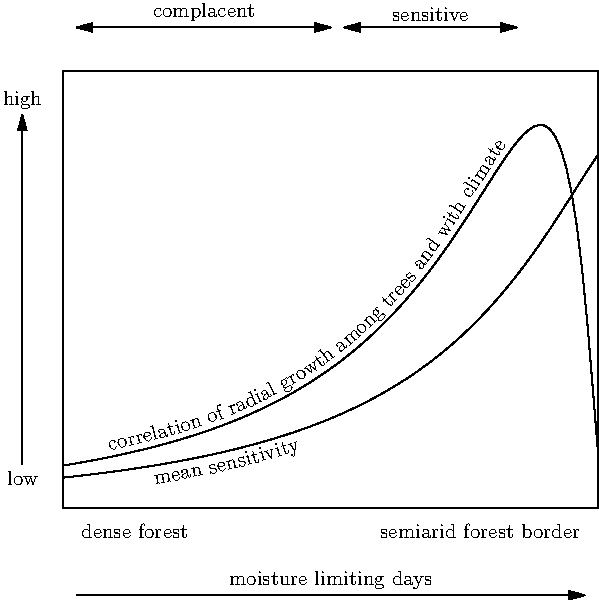
\includegraphics[width=6in]{figures/fritts.pdf}
%\caption{A simplified rendition of the diagram originally seen in \cite{fritts1976tree}.}
%\label{fig:fritts}
%\end{figure}

\begin{figure}
\centering
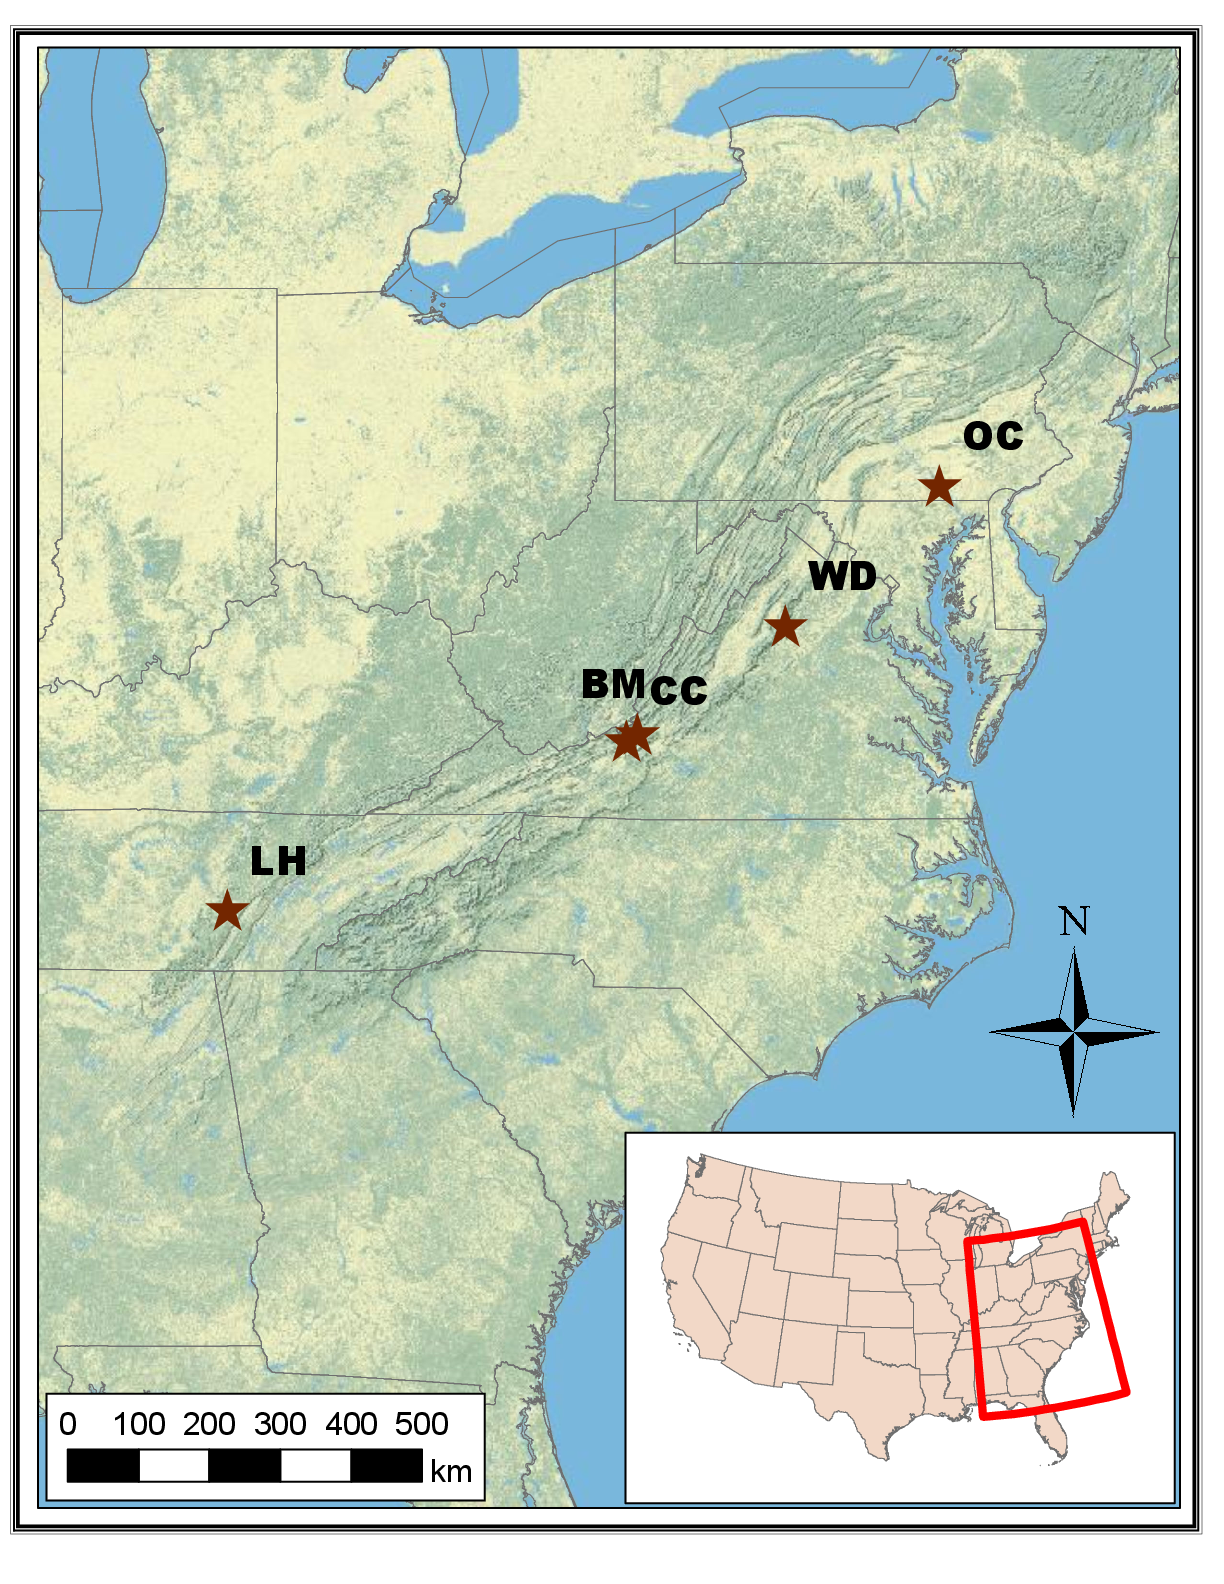
\includegraphics[width=5in]{figures/NewClimateNADEF.png}
\caption{Regional chronology sample locations.}
\label{fig:map}
\end{figure}

\begin{figure}
\centering
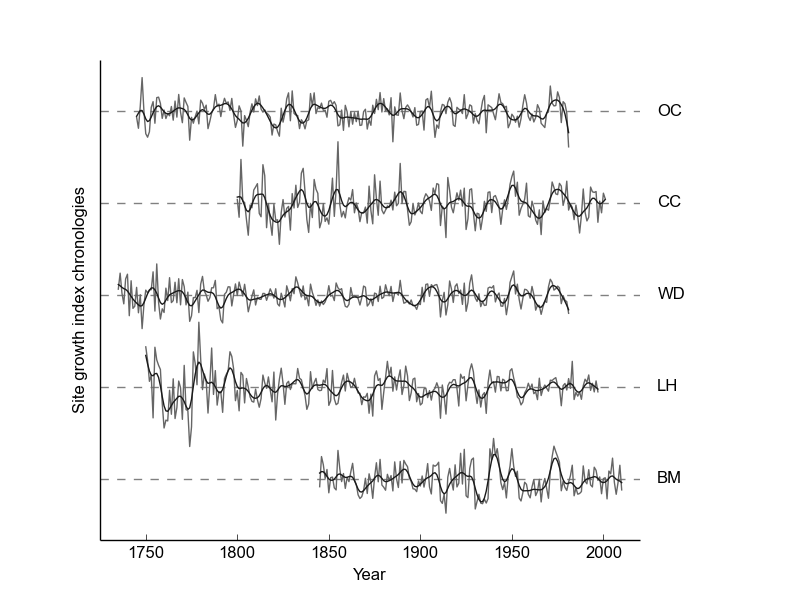
\includegraphics[width=5in]{figures/stacked_chrons.png}
\caption{Plots of the five chronologies used in the principal component analysis. The top panel shows the chronology built from the sample data at Brush Mountain (BM), while the others are the regional chronologies from Lynn Hollow (LH), watchdog Mountain (WD), Craig Creek (CC), and Otter Creek (OC).}
\label{fig:stackedChrons}
\end{figure}

\begin{figure}
\centering
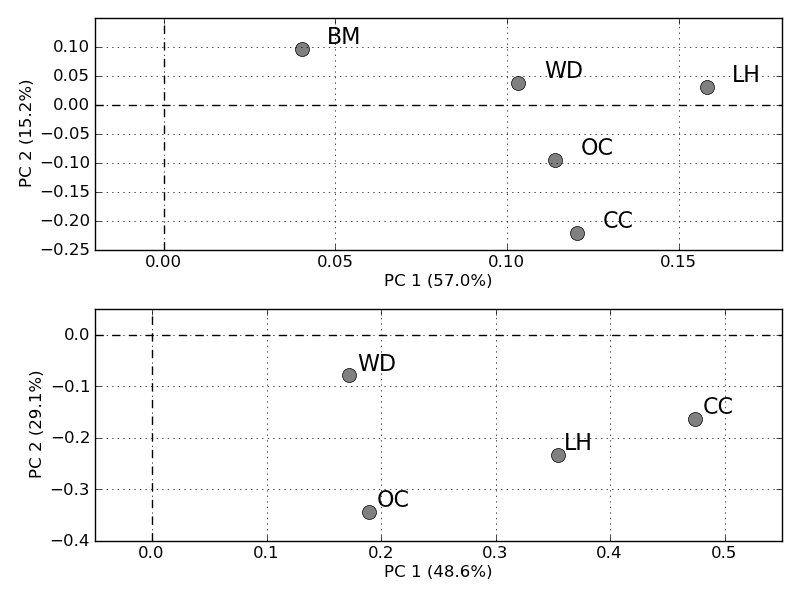
\includegraphics[width=5in]{figures/scoresPlot.png}
\caption{Top: Scatter plot of the loadings for the five chronologies analyzed in the first PCA which covered the period 1845-1981. Bottom: Scatter plot of the loadings for the five chronologies analyzed in the second PCA which covered the period 1750-1981.}
\label{fig:scores}
\end{figure}

\begin{figure}
\centering
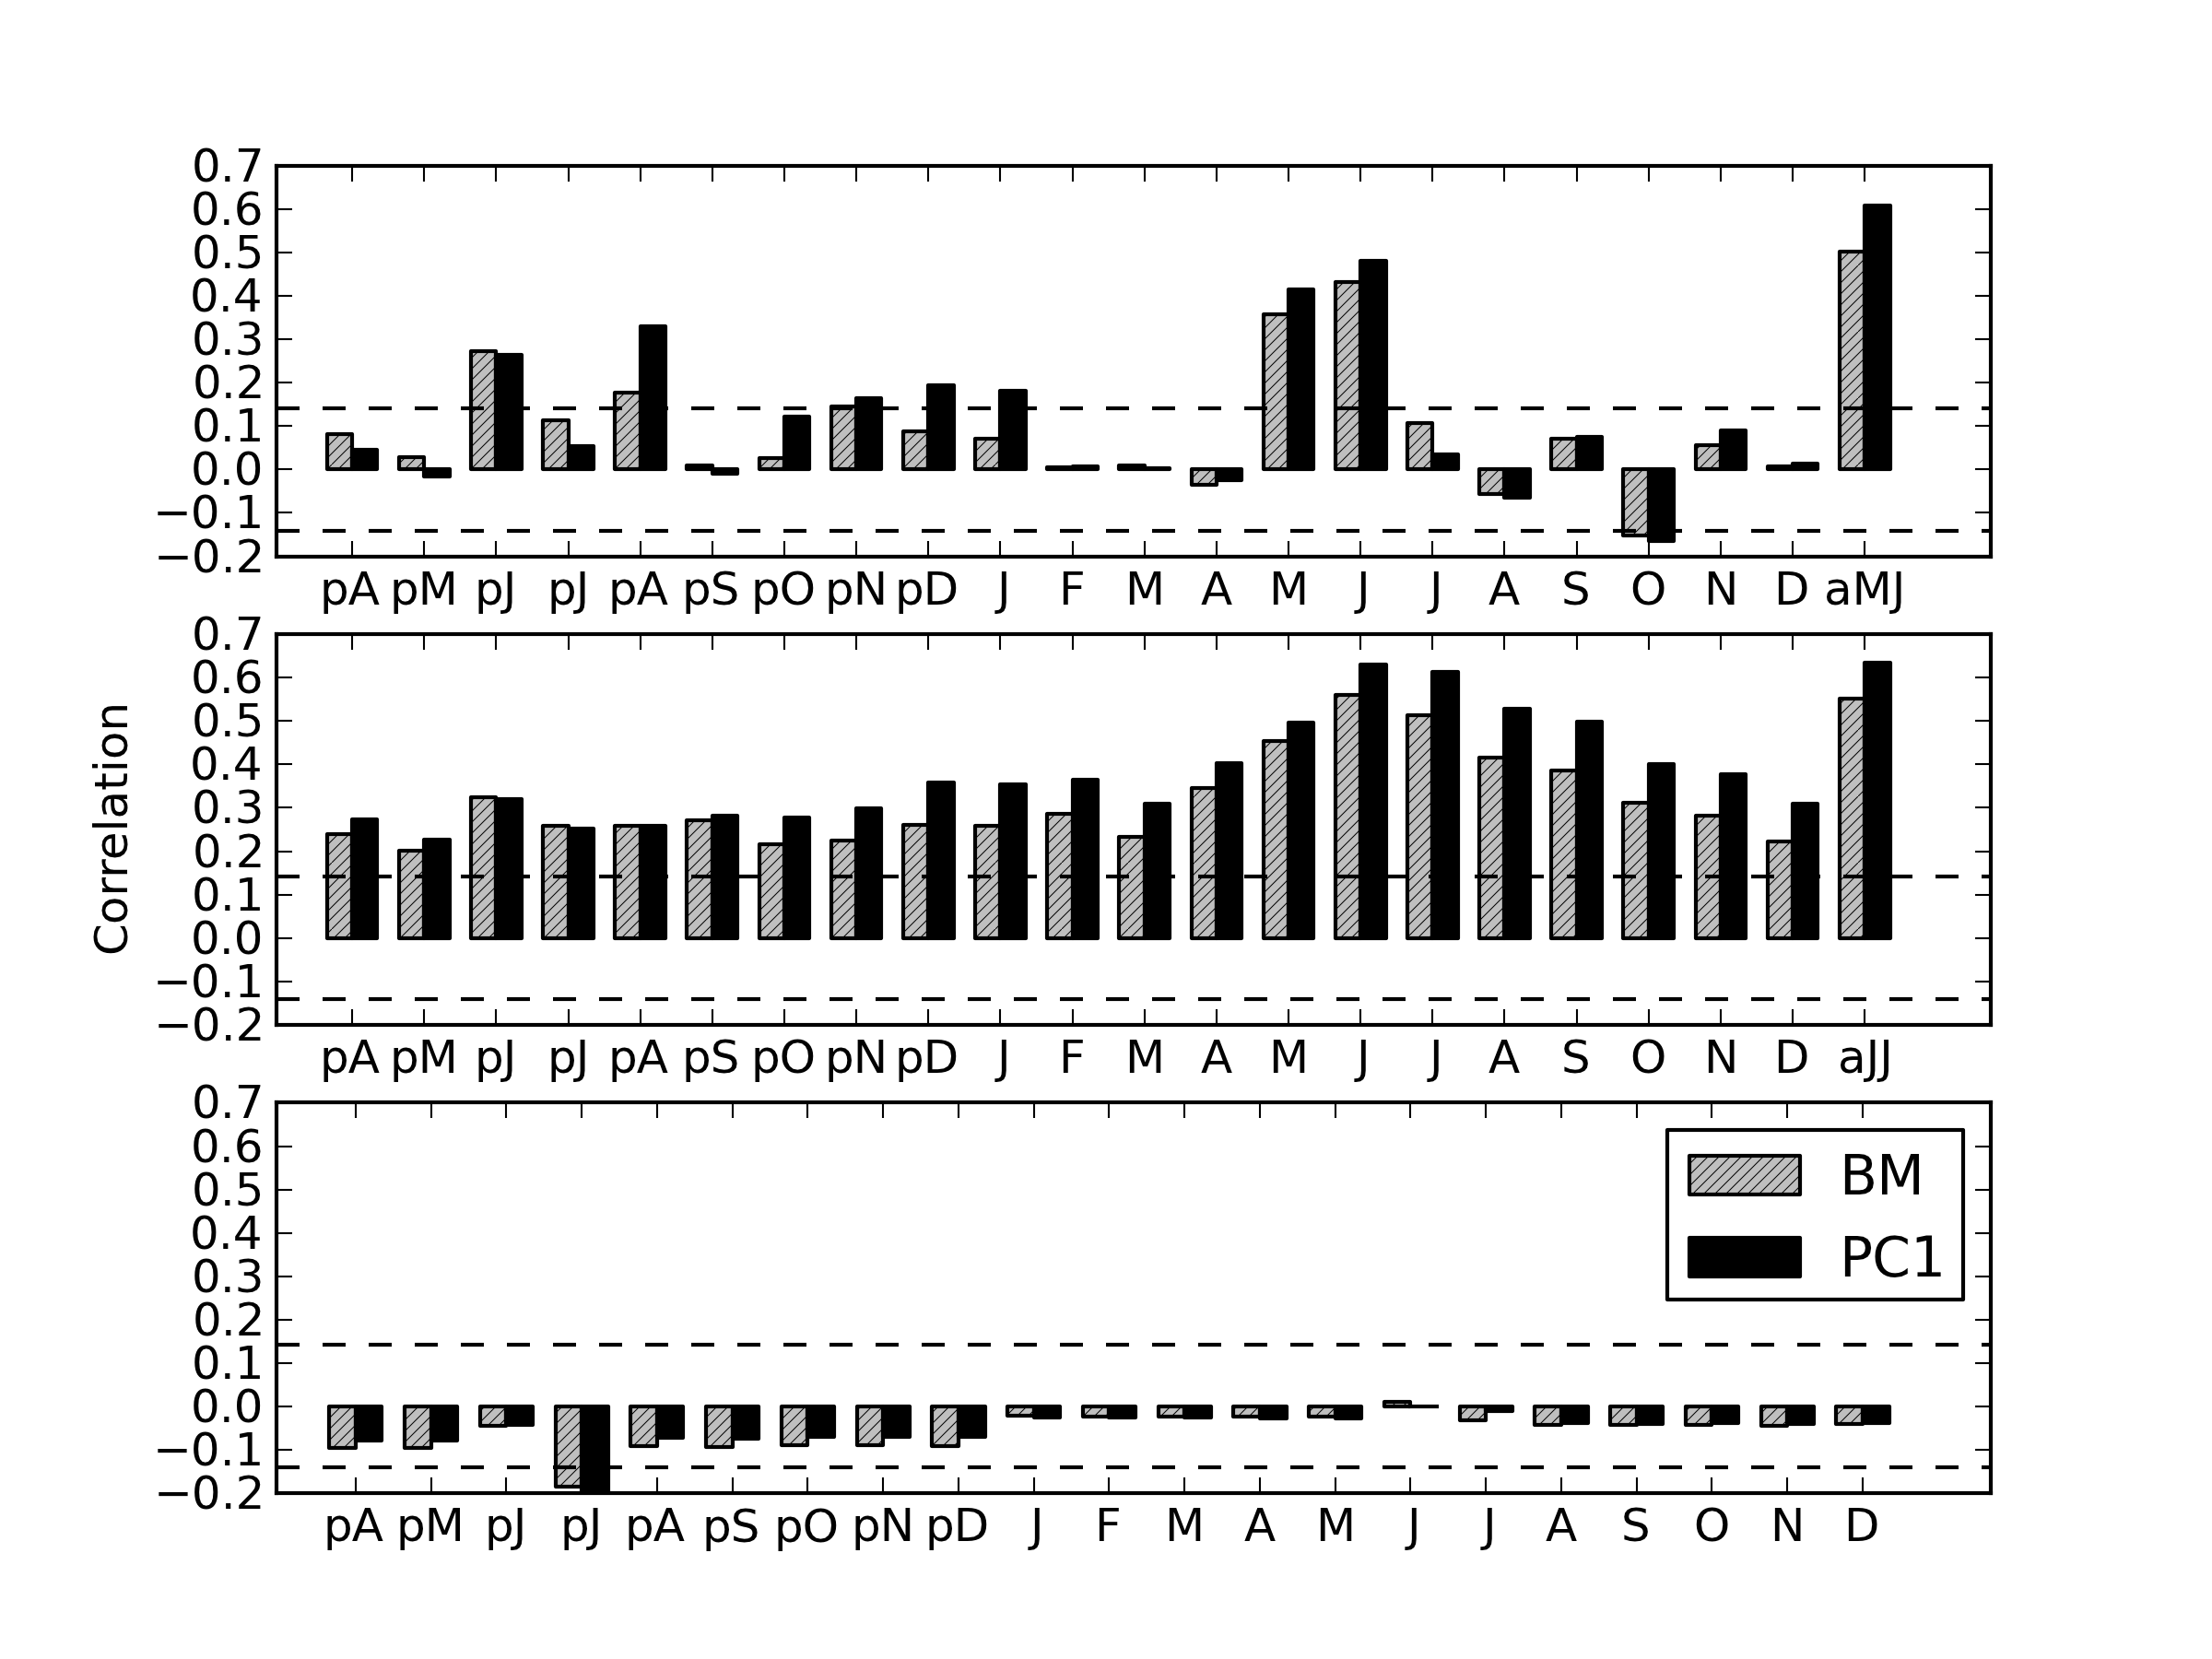
\includegraphics[width=5in]{figures/climCorr.png}
\caption{Top: Correlation between the growth proxies (BM or PC1) and the monthly precipitation from previous April (pA) through December (D) as well as for average May and June (aMJ). Middle: Correlation between the growth proxies (BM or PC1) and average PDSI from previous April (pA) through December (D) as well as for average June and July (aJJ). Bottom: Correlation between the growth proxies (BM or PC1) and average monthly temperature from previous April (pA) through December (D).}
\label{fig:climCorr}
\end{figure}

%\begin{figure}
%\centering
%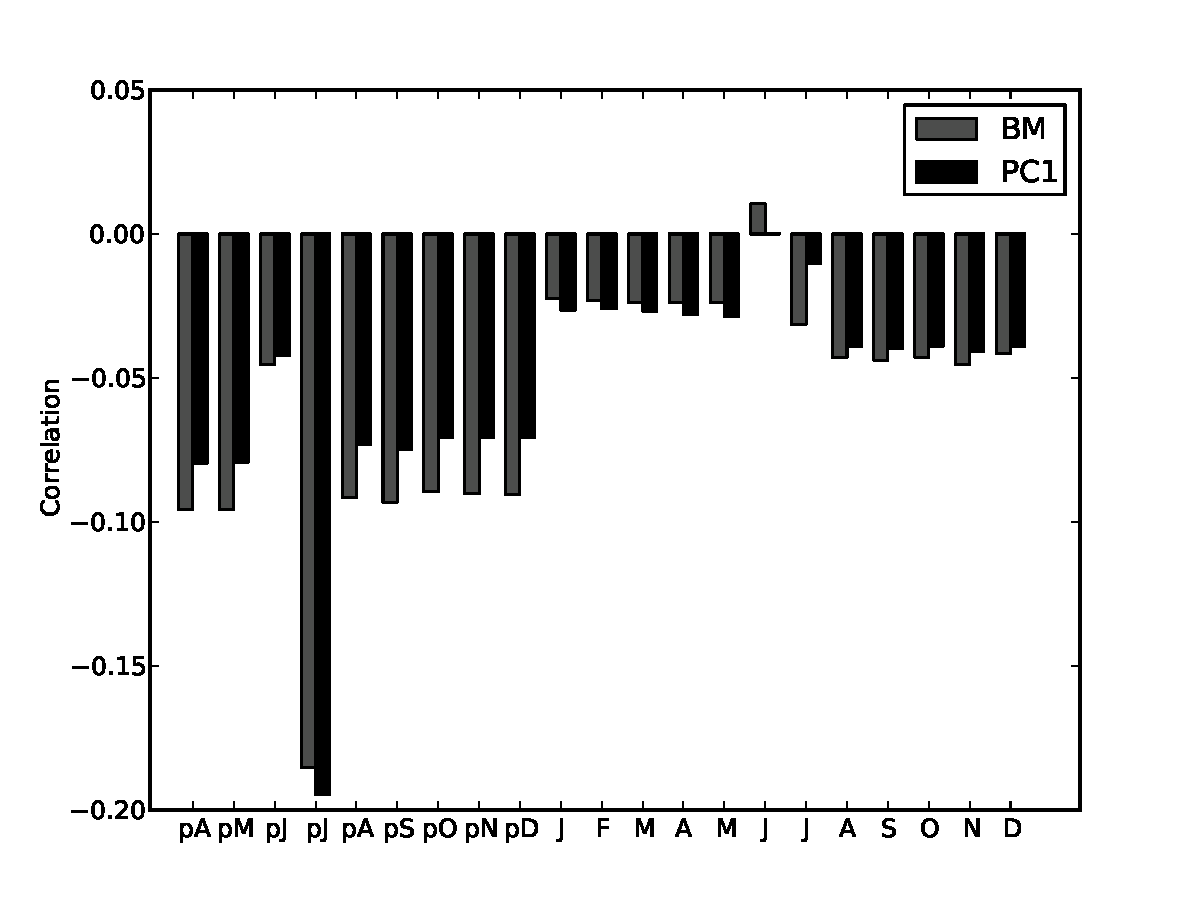
\includegraphics[width=6in]{figures/climCorrTemp.pdf}
%\caption{Correlation between the growth proxies (BM or PC1) and average monthly temperature from previous April (pA) through December (D).}
%\label{fig:tempBarCorr}
%\end{figure}

%\begin{figure}
%\centering
%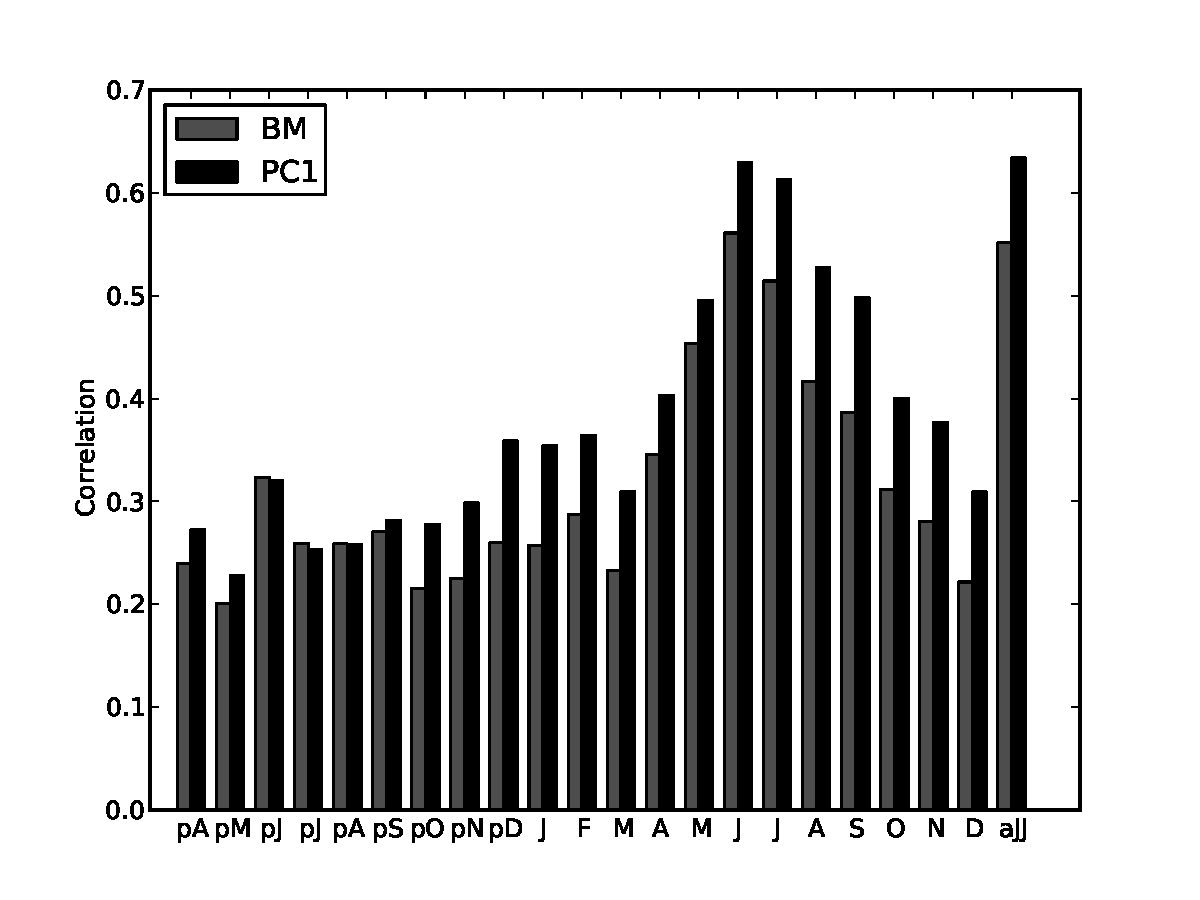
\includegraphics[width=6in]{figures/climCorrPdsi.pdf}
%\caption{Correlation between the growth proxies (BM or PC1) and average PDSI from previous April (pA) through December (D) as well as for averaged June and July (aJJ).}
%\label{fig:pdsiBarCorr}
%\end{figure}

\begin{figure}
\centering
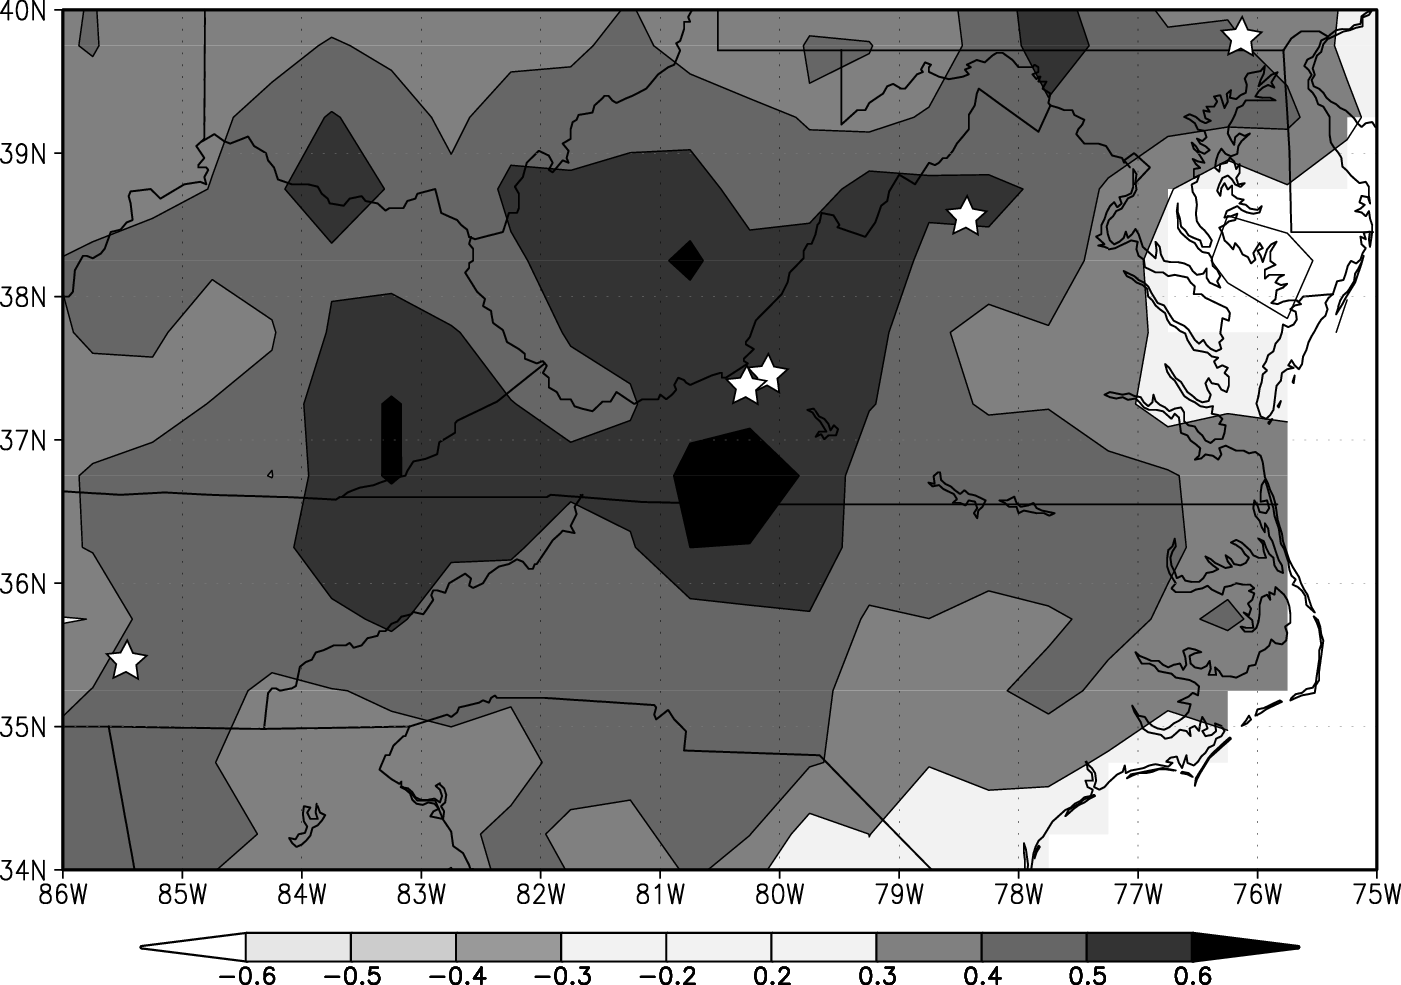
\includegraphics[width=5in]{figures/corrMapPrecipMJ_bw_annot.png}
\caption{Correlation map showing the correlation between the first principal component and averaged May-June precipitation. Stars indicate the locations of the sites where the tree-rings used to develop the contributing chronologies were sampled.}
\label{fig:precipCorrMap}
\end{figure}

%\begin{figure}
%\centering
%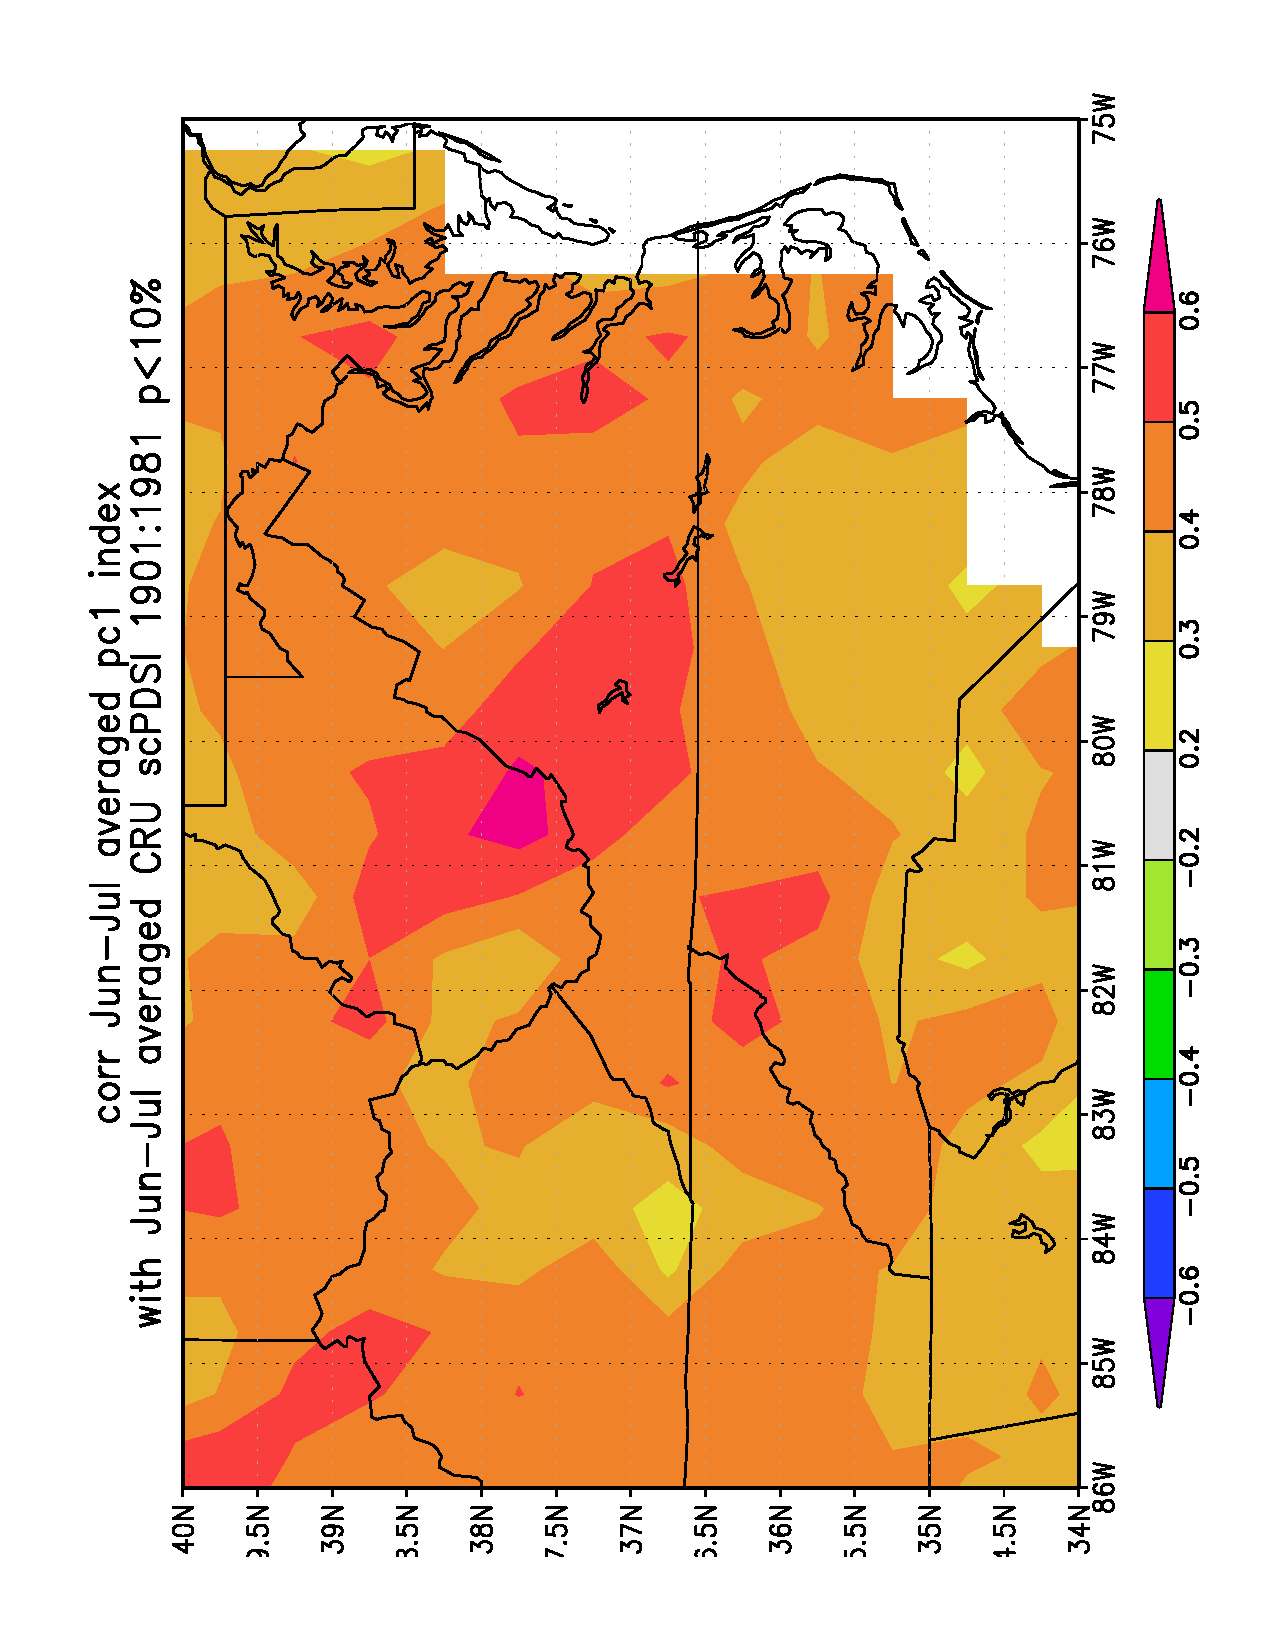
\includegraphics[width=5in, angle=-90]{figures/corrMapPdsiJJ.pdf}
%\caption{Correlation map.}
%\label{fig:pdsiCorrMap}
%\end{figure}
%
%\begin{figure}
%\centering
%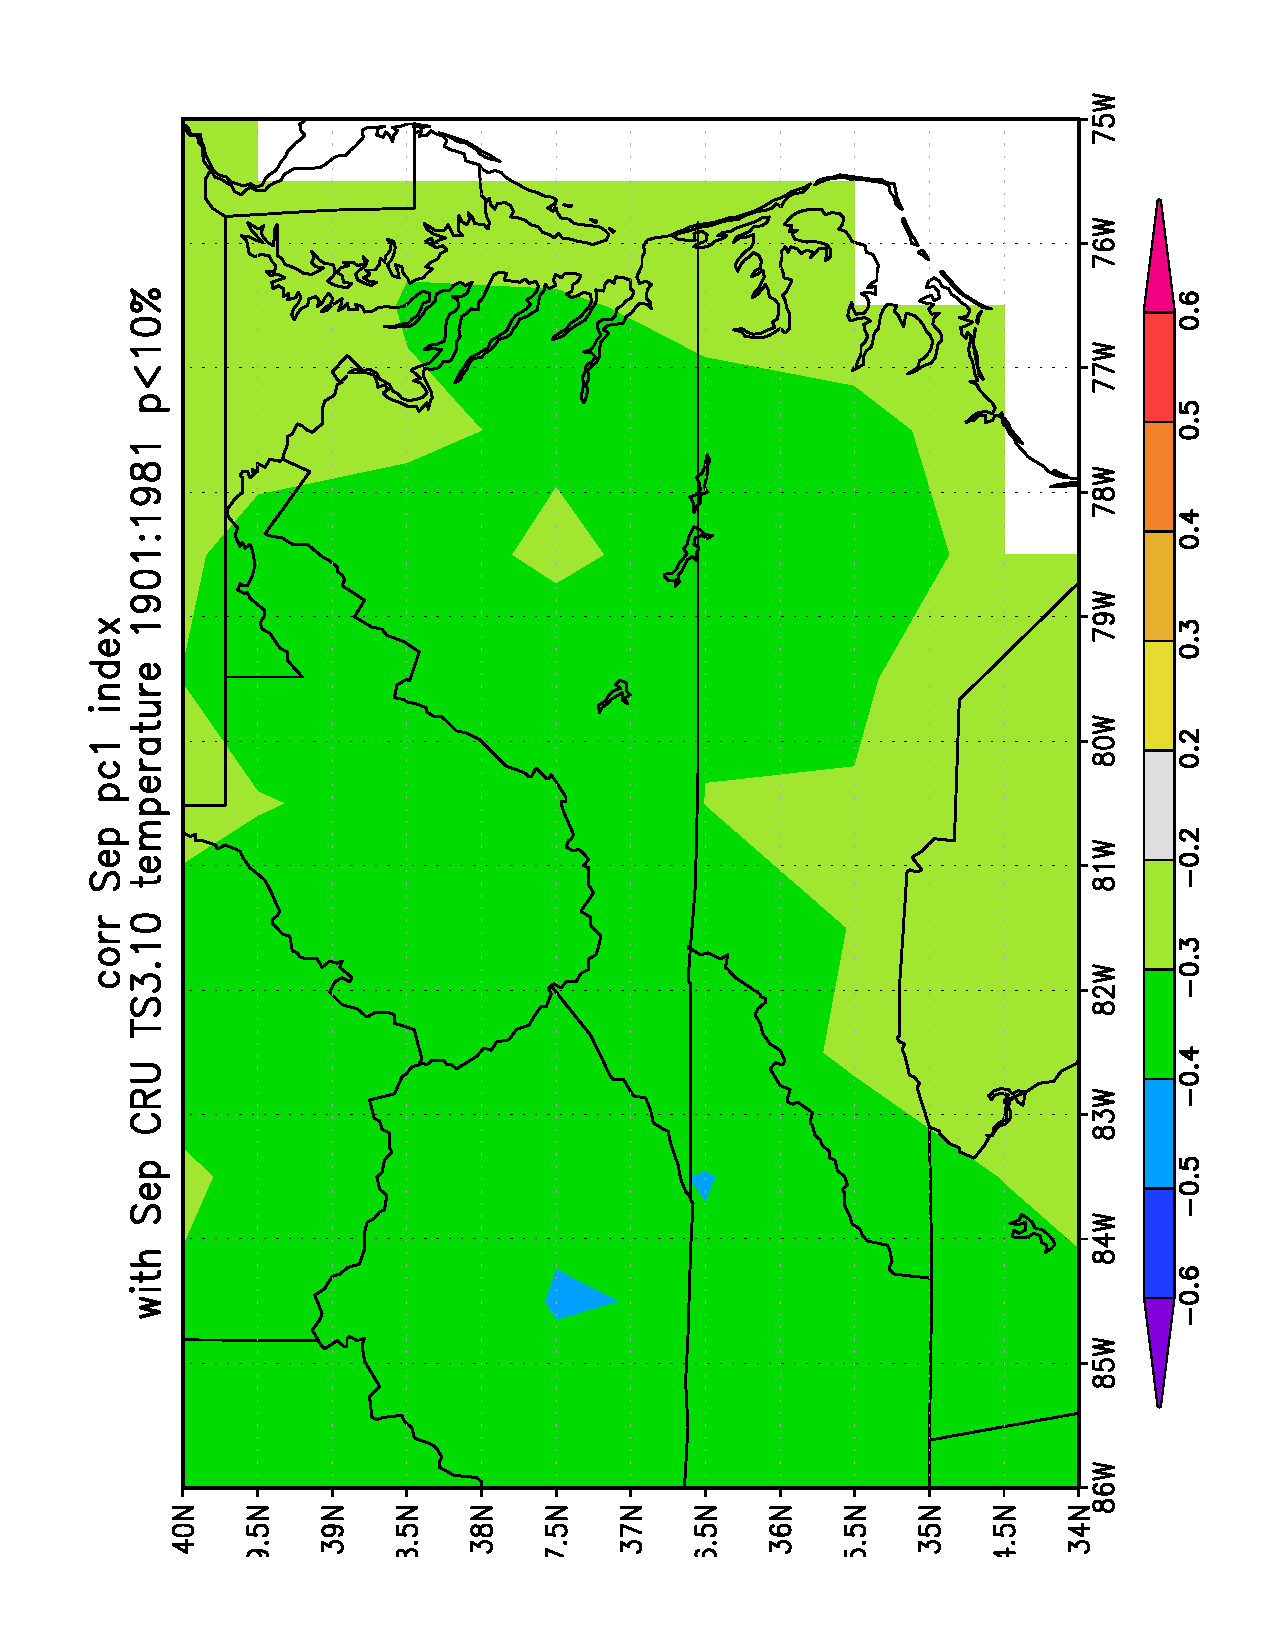
\includegraphics[width=5in, angle=-90]{figures/corrMapTempSept.pdf}
%\caption{Correlation map showing the correlation between the first principal component and September temperature.}
%\label{fig:tempCorrMap}
%\end{figure}

\begin{figure}
\centering
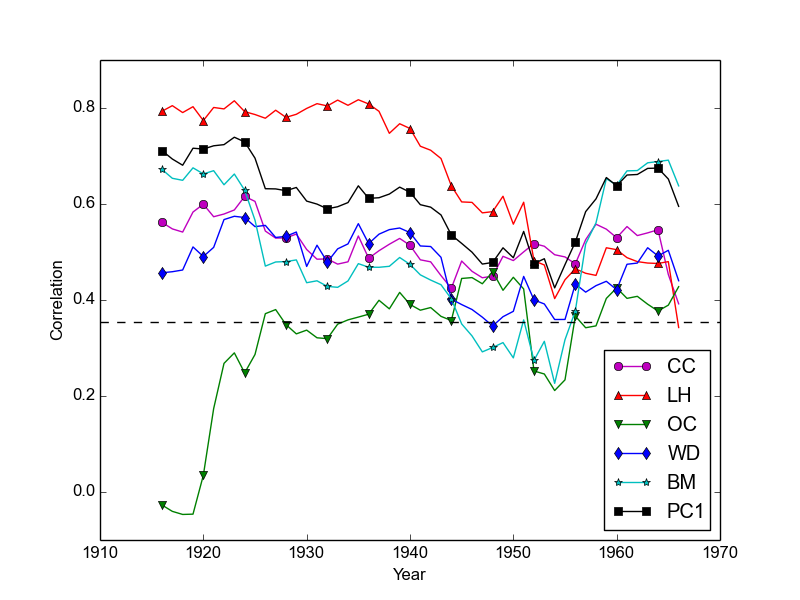
\includegraphics[width=5in]{figures/precipRunningCorr.png}
\caption{A 31-year windowed correlation plot showing the correlations between each growth proxy (chronologies and first principal component) and mjPR. Correlation points are plotted above the window centers.}
\label{fig:precipRunningCorr}
\end{figure}

\begin{figure}
\centering
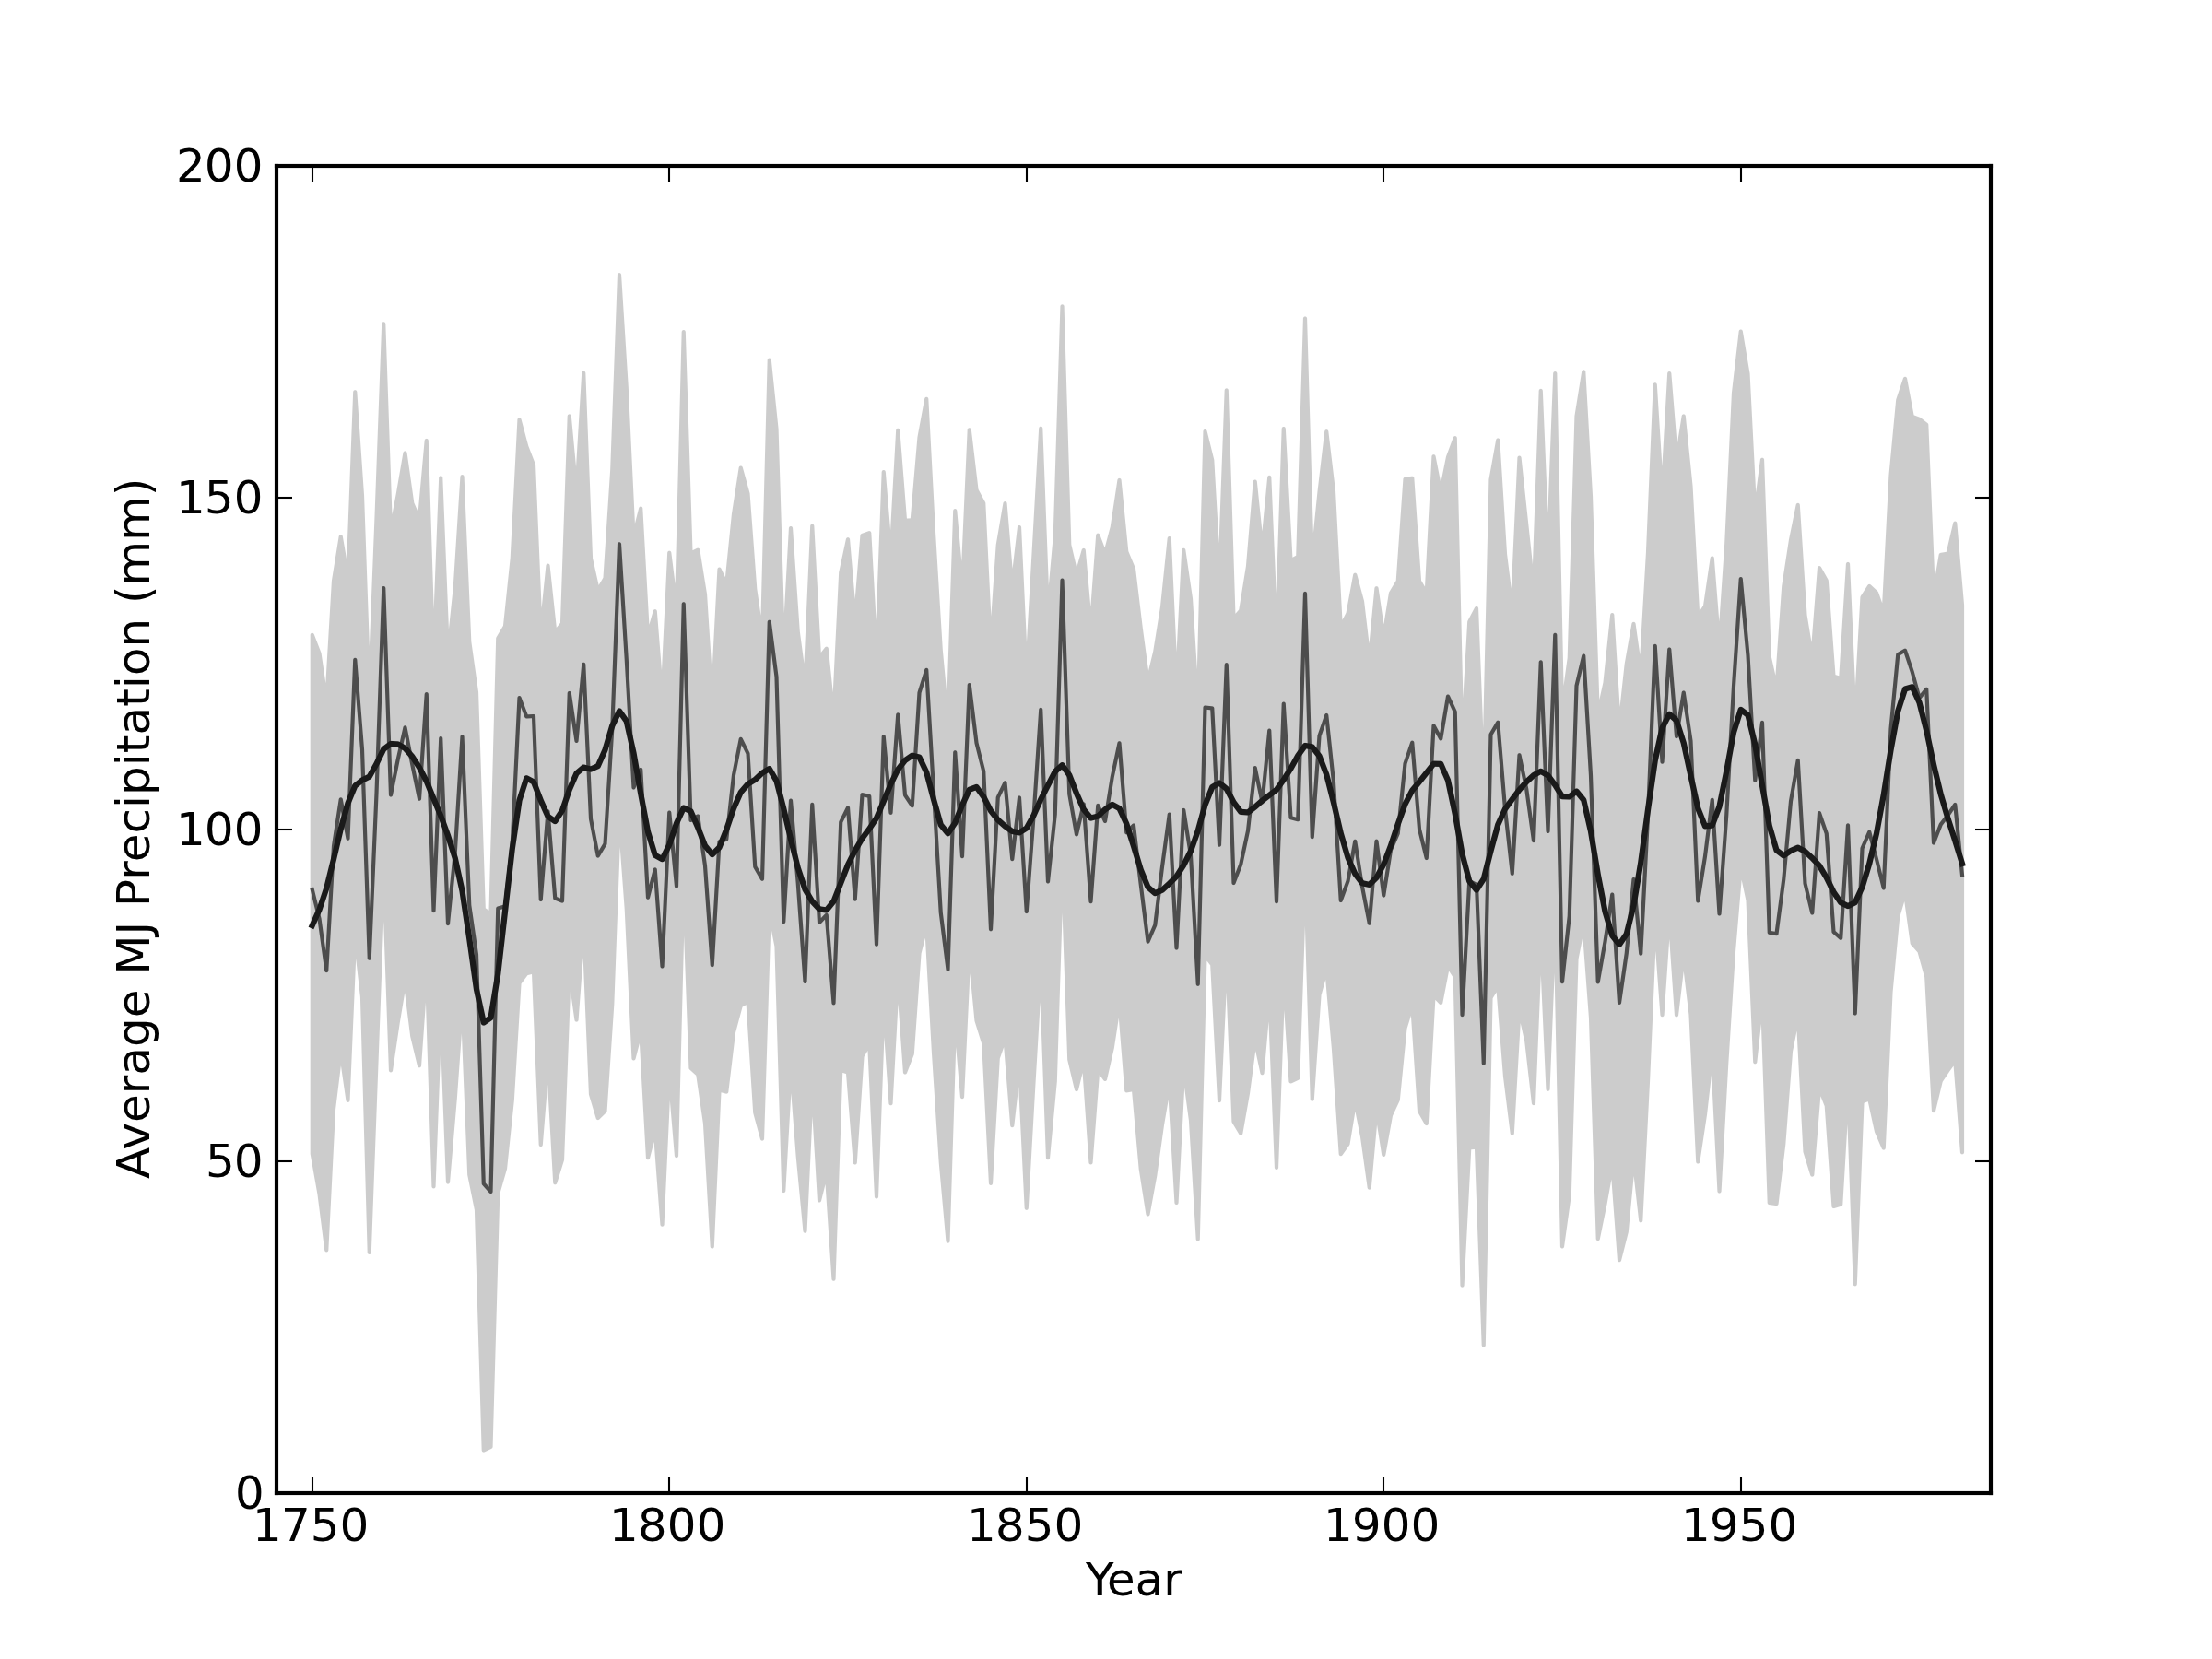
\includegraphics[width=5in]{figures/recon.png}
\caption{Average May-June precipitation (mjPR) reconstruction (grey curve), smoothed estimate showing decadal-scale variable (black curve), and the reconstruction 95\% credible interval (shaded grey region).}
\label{fig:precipRecon}
\end{figure}

\begin{figure}
\centering
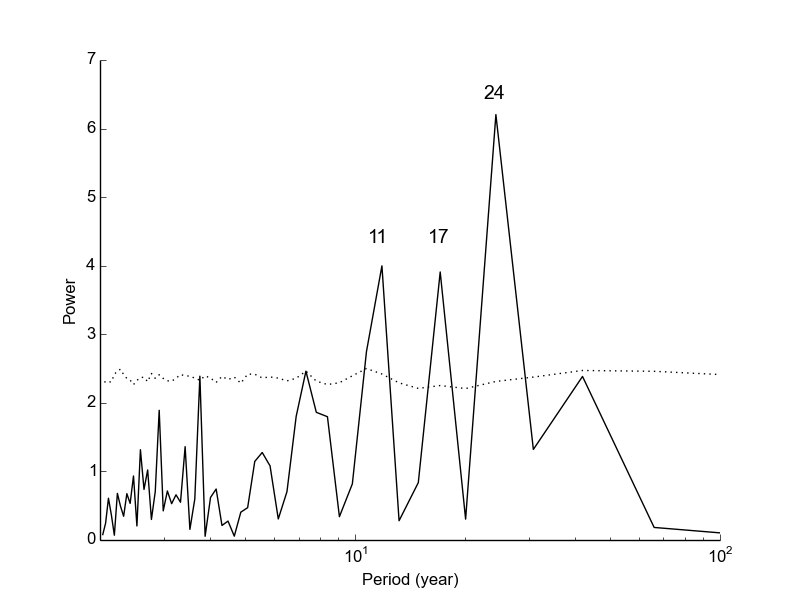
\includegraphics[width=5in]{figures/spectralRecon.png}
\caption{Periodogram showing periodicity of high amplitude at approximately 11, 17, and 24 years.}
\label{fig:spectral}
\end{figure}

\begin{figure}
\centering
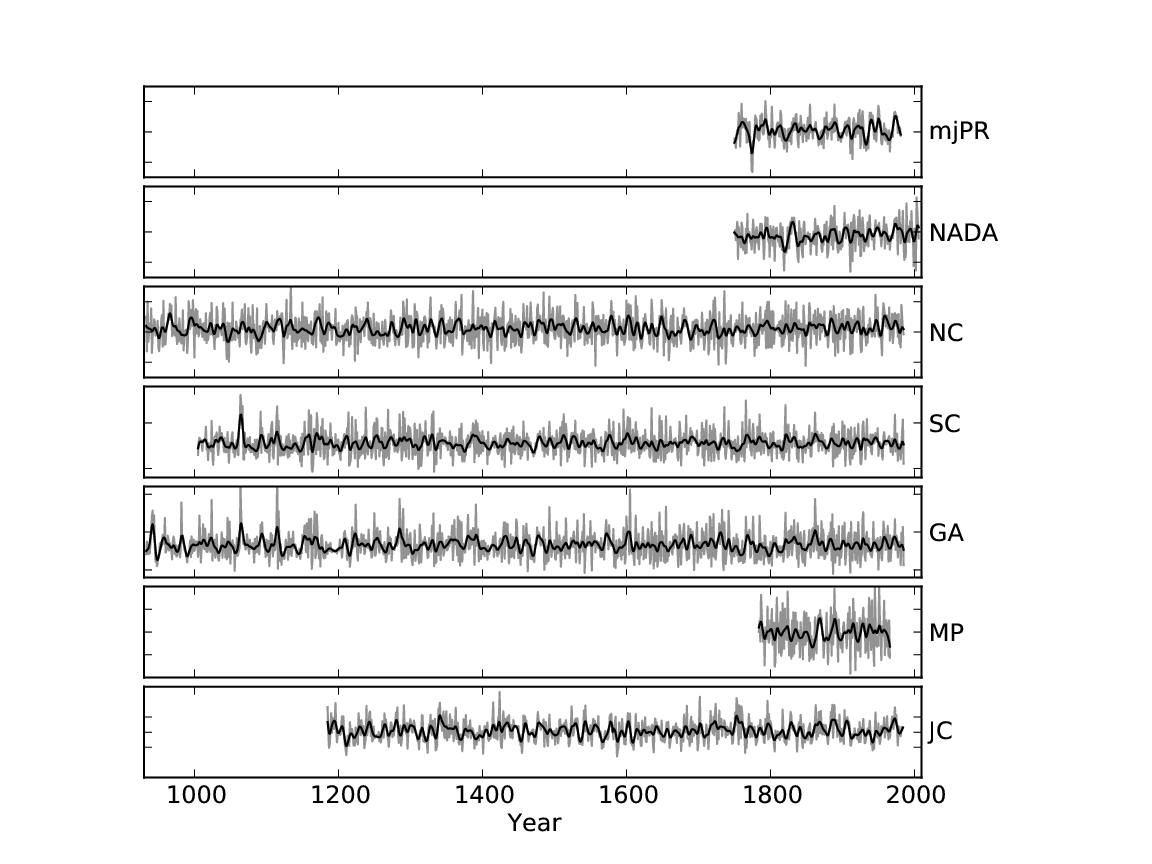
\includegraphics[width=5in]{figures/reconsStacked.png}
\caption{Time series plots showing annual- and decadal-scale variability for the mjPR and six compared moisture reconstructions for the period 933-2008.}
\label{fig:allRecons}
\end{figure}

\begin{figure}
\centering
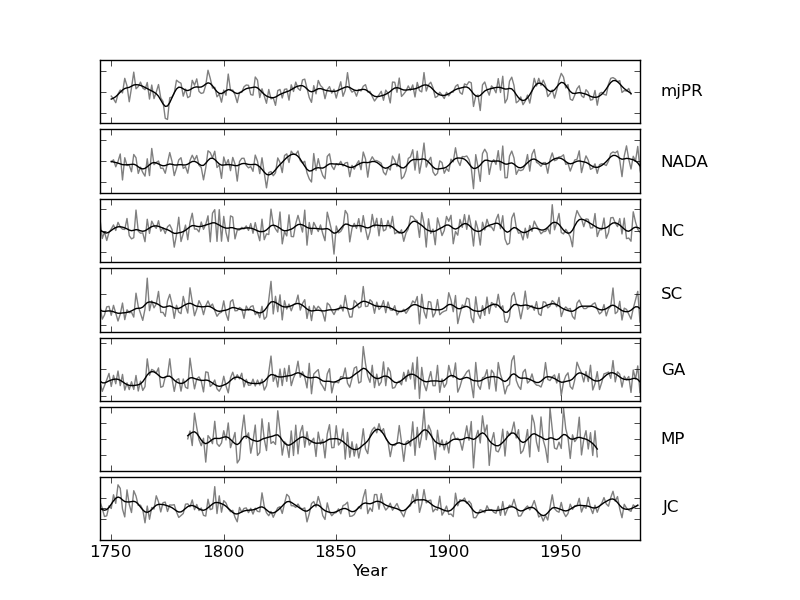
\includegraphics[width=5in]{figures/reconsStackedZoom.png}
\caption{Time series plots showing annual- and decadal-scale variability for the mjPR and six compared moisture reconstructions for the period 1745-1985.}
\label{fig:allReconsZoom}
\end{figure}


\begin{figure}
\centering
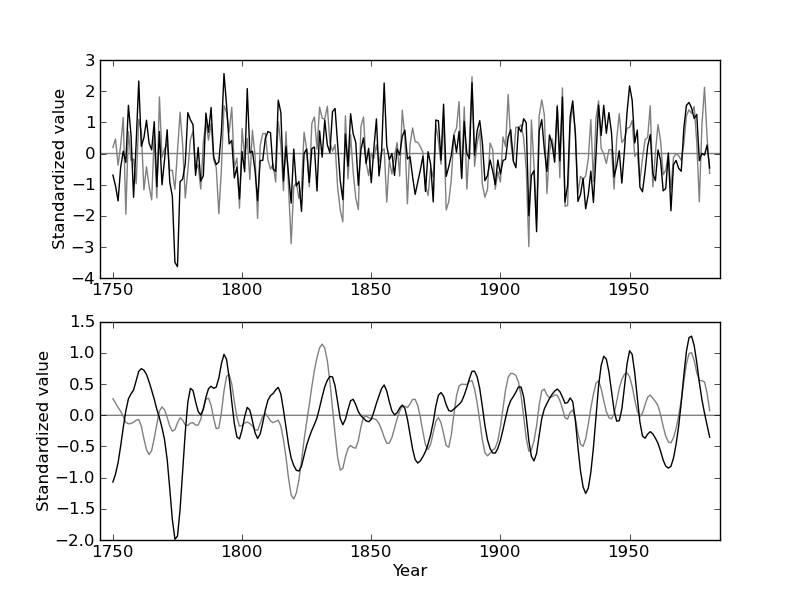
\includegraphics[width=5in]{figures/reconCompare.png}
\caption{Both the mjPR reconstruction and the Cook PDSI reconstruction are standardized and plotted against time to highlight both the similarities and the differences. Particularly notable differences include the year 1774, and the interval 1855-1863.}
\label{fig:reconCompare}
\end{figure}

\begin{figure}
\centering
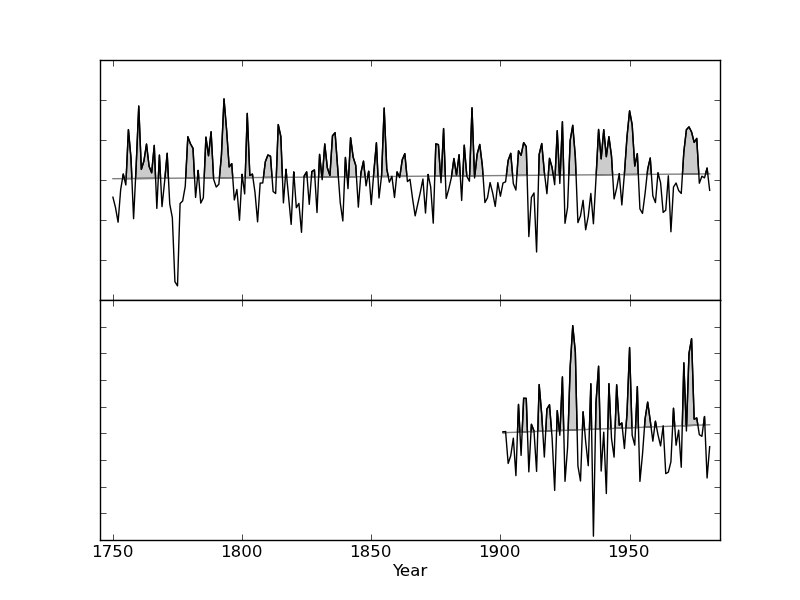
\includegraphics[width=5in]{figures/wetdry.png}
\caption{The mjPR reconstruction (top panel) and the mjPR instrumental record (bottom panel). Lines show the best-fit regression line through the time series data to indicate any dominant trends. Areas falling above the best-fit lines and the time series data are shaded grey to indicate periods of higher precipitation. Note the correspondence of wetter and drier years between the top and bottom panels.}
\label{fig:wetdry}
\end{figure}

\begin{figure}
\centering
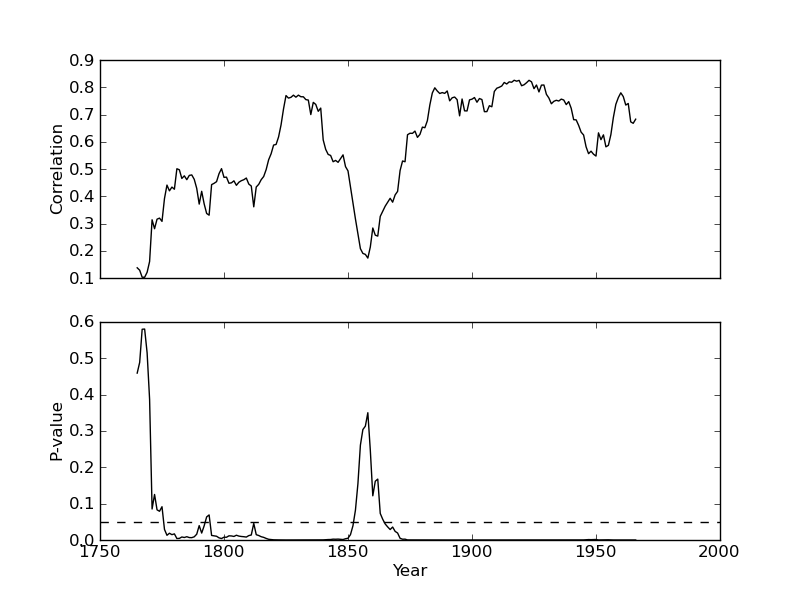
\includegraphics[width=5in]{figures/reconRunningCorr.png}
\caption{A 31 year windowed correlation plot between the mjPR and Cook PDSI reconstructions shows the discrepancy during the 1855-1863 interval. In the top panel correlation values are plotted about window centers, while the bottom panel shows the corresponding p-value (black) as well as the line of significance (dashed).}
\label{fig:reconRunningCorr}
\end{figure}

\begin{figure}
\centering
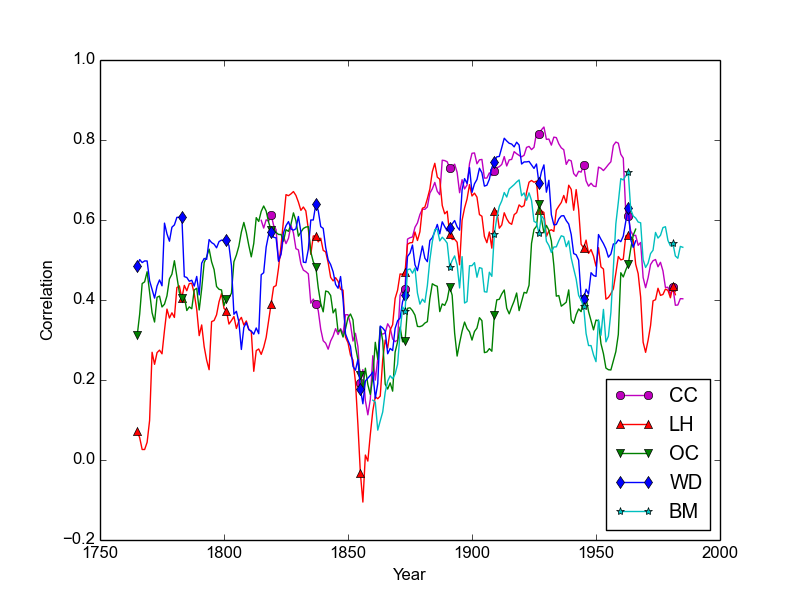
\includegraphics[width=5in]{figures/cookPdsiRunningCorr.png}
\caption{A 31 year windowed correlation plot between each of the chronologies and the Cook PDSI reconstruction. Note the interval of abrupt poor correlation during the years 1855-1863.}
\label{fig:cookRunningPdsiCorr}
\end{figure}



%%
%% reference
%%

\newpage
\clearpage
\bibliographystyle{unsrtnat}
\bibliography{oakRecon}

\end{document}
